\begin{table}[t]
	\caption{Throughput: Operations/Lots across different Planning Hours} \label{tab:my_label} \centering
	\begin{tabular}{|l|c|c|c|c|c|c|}
		\hline
		\textbf{Algorithm} & \textbf{1} & \textbf{2} & \textbf{3} & \textbf{4} & \textbf{5} & \textbf{6} \\ \cline{1-7} 
		Dispatcher (fifo)   & 1819/0 & 2846/0 & 4027/1 & 4916/4 & 5956/6 & 6822/8 \\
		Dispatcher (cr)     & 1801/0 & 2830/0 & 4028/1 & 4933/3 & 5994/5 & 6934/8 \\
		Dispatcher (random) & 1809/0 & 2884/0 & 4102/1 & 4976/3 & 6045/5 & 6954/7 \\
		Scheduler (gsaco)   & 1847/0 & 2960/0 & 4093/1 & 4970/3 & 5975/5 & 6716/7 \\
		\hline 
	\end{tabular}
\end{table}


\begin{table}[t]
	\caption{Percentage Change in Dispatcher Performance Over Planning Hours (HV/LM)} \label{tab:dispatchers} \centering
	\begin{tabular}{|l|c|c|c|c|c|c|}
		\hline
		\textbf{Dispatcher} & \textbf{1} & \textbf{2} & \textbf{3} & \textbf{4} & \textbf{5} & \textbf{6} \\
		\hline 
		FIFO     & -    & -    & -    & -    & -    & -    \\
		CR       & -0.99\% & -0.56\% & 0.02\% & 0.35\% & 0.64\% & 1.64\% \\
		RANDOM   & -0.55\% & 1.33\% & 1.86\% & 1.22\% & 1.49\% & 1.93\% \\
		GSACO    & 0.72\% & 1.93\% & 3.43\% & 3.03\% & 2.19\% & 1.70\% \\
		\hline
	\end{tabular}
\end{table}

\begin{table}[t]
	\caption{FJSSP results obtained with CP and GSACO}\label{tab:benchmarkresults} \centering
	\begin{tabular}{|lr|r|r|r|}
		\hline
		Instance & $J$  & $M$ & CP  & GSACO \\ \hline
		MK1      & $10$ & $6$ & $40$  & $44$     \\ 
		MK2      & $10$ & $6$ & $27$  & $40$     \\ 
		MK3      & $15$ & $8$ & $204$ & $239$    \\ 
		MK4      & $15$ & $8$ & $60$  & $83$     \\ 
		SFJSSP1   & $2$ & $2$ & $66$  & $66$     \\ 
		SFJSSP2   & $2$ & $2$ & $107$ & $107$    \\ 
		SFJSSP3   & $3$ & $2$ & $221$ & $221$    \\ 
		SFJSSP4   & $3$ & $2$ & $355$ & $355$    \\ 
		MFJSSP1   & $5$ & $6$ & $468$ & $498$    \\ 
		MFJSSP2   & $5$ & $7$ & $446$ & $470$    \\ 
		MFJSSP3   & $6$ & $7$ & $466$ & $523$    \\ 
		MFJSSP4   & $7$ & $7$ & $554$ & $664$    \\ 
		\hline
	\end{tabular}
\end{table}



\begin{table}[t]
	\caption{SMSP results obtained with GSACO-O}	\label{tab:results-operations} \centering
	\begin{tabular}{|l|cccccc|}
		\hline
		\multicolumn{1}{|c|}{\multirow{2}{*}{Instance}} &
		\multicolumn{6}{c|}{Planning period in hours} \\ \cline{2-7} 
		\multicolumn{1}{|c|}{} &
		\multicolumn{1}{c|}{1} &
		\multicolumn{1}{c|}{2} &
		\multicolumn{1}{c|}{3} &
		\multicolumn{1}{c|}{4} &
		\multicolumn{1}{c|}{5} &
		6 \\ \hline &
		\multicolumn{1}{l|}{Ops/Lots} &
		\multicolumn{1}{l|}{Ops/Lots} &
		\multicolumn{1}{l|}{Ops/Lots} &
		\multicolumn{1}{l|}{Ops/Lots} &
		\multicolumn{1}{c|}{Ops/Lots} &
		\multicolumn{1}{l|}{Ops/Lots} \\ \cline{2-7}
		LV/HM &
		\multicolumn{1}{c|}{1422/0} &
		\multicolumn{1}{c|}{2368/0} &
		\multicolumn{1}{c|}{3234/0} &
		\multicolumn{1}{c|}{4015/1} &
		\multicolumn{1}{c|}{4722/2} &
		5306/2 \\ 
		HV/LM &
		\multicolumn{1}{c|}{1848/0} &
		\multicolumn{1}{c|}{2960/0} &
		\multicolumn{1}{c|}{4093/1} &
		\multicolumn{1}{c|}{4970/3} &
		\multicolumn{1}{c|}{5975/5} &
		6716/7 \\ \hline
	\end{tabular}%
\end{table}


\begin{table}[t]
	\caption{Percentage Change in Dispatcher Performance Over Planning Hours (HV/LM)}\label{tab:dispatchers-HVLM} 
	\begin{tabular}{|l|cccccccccccc|}
		\hline
		\multirow{3}{*}{Dispatcher} &
		\multicolumn{12}{c|}{Planning period in hours} \\ \cline{2-13} 
		&
		\multicolumn{2}{c|}{1} &
		\multicolumn{2}{c|}{2} &
		\multicolumn{2}{c|}{3} &
		\multicolumn{2}{c|}{4} &
		\multicolumn{2}{c|}{5} &
		\multicolumn{2}{c|}{6} \\ \cline{2-13} 
		&
		\multicolumn{1}{l|}{Ops/Lots} &
		\multicolumn{1}{l|}{\% change} &
		\multicolumn{1}{l|}{Ops/Lots} &
		\multicolumn{1}{l|}{\% change} &
		\multicolumn{1}{l|}{Ops/Lots} &
		\multicolumn{1}{l|}{\% change} &
		\multicolumn{1}{l|}{Ops/Lots} &
		\multicolumn{1}{l|}{\% change} &
		\multicolumn{1}{l|}{Ops/Lots} &
		\multicolumn{1}{l|}{\% change} &
		\multicolumn{1}{l|}{Ops/Lots} &
		\multicolumn{1}{l|}{\% change} \\ \hline 
		FIFO &
		\multicolumn{1}{c|}{1821/0} &
		\multicolumn{1}{c|}{-} &
		\multicolumn{1}{c|}{2831/0} &
		\multicolumn{1}{c|}{-} &
		\multicolumn{1}{c|}{4020/1} &
		\multicolumn{1}{c|}{-} &
		\multicolumn{1}{c|}{4914/4} &
		\multicolumn{1}{c|}{-} &
		\multicolumn{1}{c|}{5960/6} &
		\multicolumn{1}{c|}{-} &
		\multicolumn{1}{c|}{6841/8} &
		- \\
		CR &
		\multicolumn{1}{c|}{1798/0} &
		\multicolumn{1}{c|}{-1.26\%} &
		\multicolumn{1}{c|}{2811/0} &
		\multicolumn{1}{c|}{-0.71\%} &
		\multicolumn{1}{c|}{4021/1} &
		\multicolumn{1}{c|}{0.02\%} &
		\multicolumn{1}{c|}{4934/3} &
		\multicolumn{1}{c|}{0.40\%} &
		\multicolumn{1}{c|}{6003/5} &
		\multicolumn{1}{c|}{0.72\%} &
		\multicolumn{1}{c|}{6946/8} &
		1.53\% \\
		RANDOM &
		\multicolumn{1}{c|}{1810/0} &
		\multicolumn{1}{c|}{-0.60\%} &
		\multicolumn{1}{c|}{2852/0} &
		\multicolumn{1}{c|}{0.74\%} &
		\multicolumn{1}{c|}{4065/1} &
		\multicolumn{1}{c|}{1.12\%} &
		\multicolumn{1}{c|}{4975/3} &
		\multicolumn{1}{c|}{1.24\%} &
		\multicolumn{1}{c|}{6026/5} &
		\multicolumn{1}{c|}{1.10\%} &
		\multicolumn{1}{c|}{6973/9} &
		1.92\% \\
		GSACO &
		\multicolumn{1}{c|}{1831/0} &
		\multicolumn{1}{c|}{0.54\%} &
		\multicolumn{1}{c|}{2957/0} &
		\multicolumn{1}{c|}{4.45\%} &
		\multicolumn{1}{c|}{4162/1} &
		\multicolumn{1}{c|}{3.53\%} &
		\multicolumn{1}{c|}{5118/3} &
		\multicolumn{1}{c|}{4.15\%} &
		\multicolumn{1}{c|}{6263/5} &
		\multicolumn{1}{c|}{5.08\%} &
		\multicolumn{1}{c|}{7162/7} &
		4.69\% \\ \hline
	\end{tabular}%
\end{table}

\begin{figure}[ht]
	\centering
	\begin{subfigure}{0.32\textwidth}
		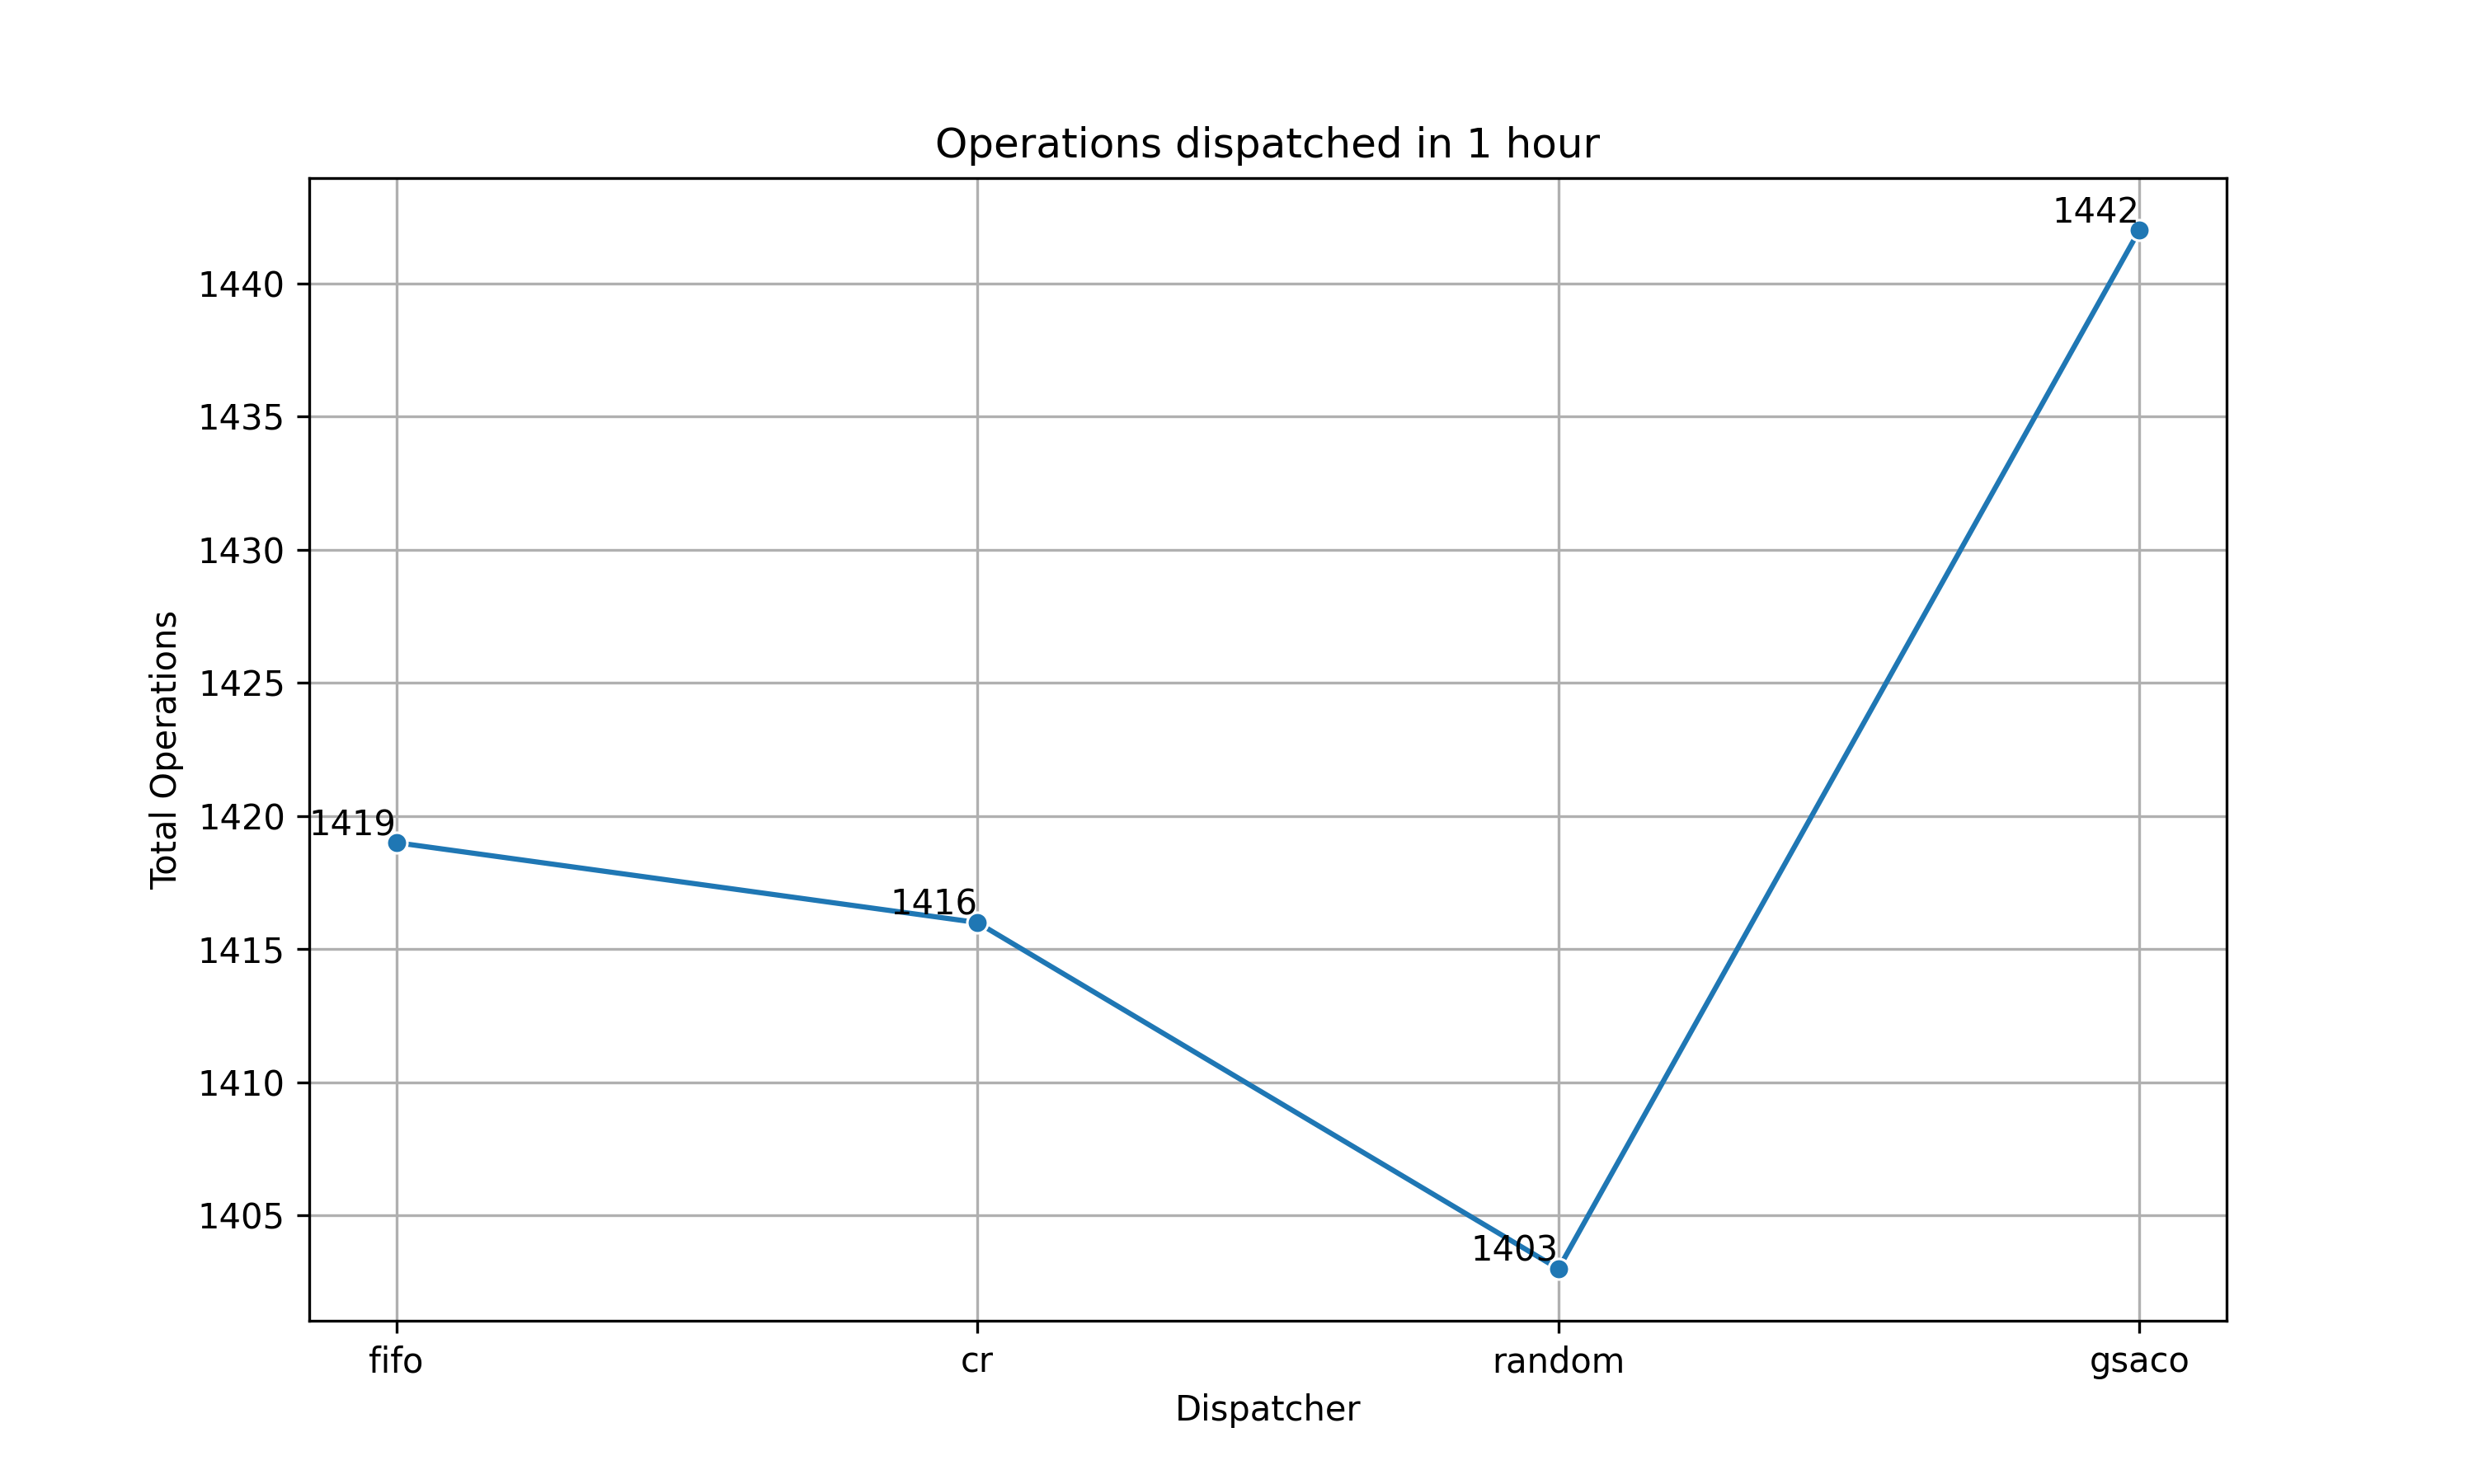
\includegraphics[width=\textwidth]{LVHM/total_operations_3600s.png}
		% \caption{}
		% \label{fig:oo1}
	\end{subfigure}\hfill
	\begin{subfigure}{0.32\textwidth}
		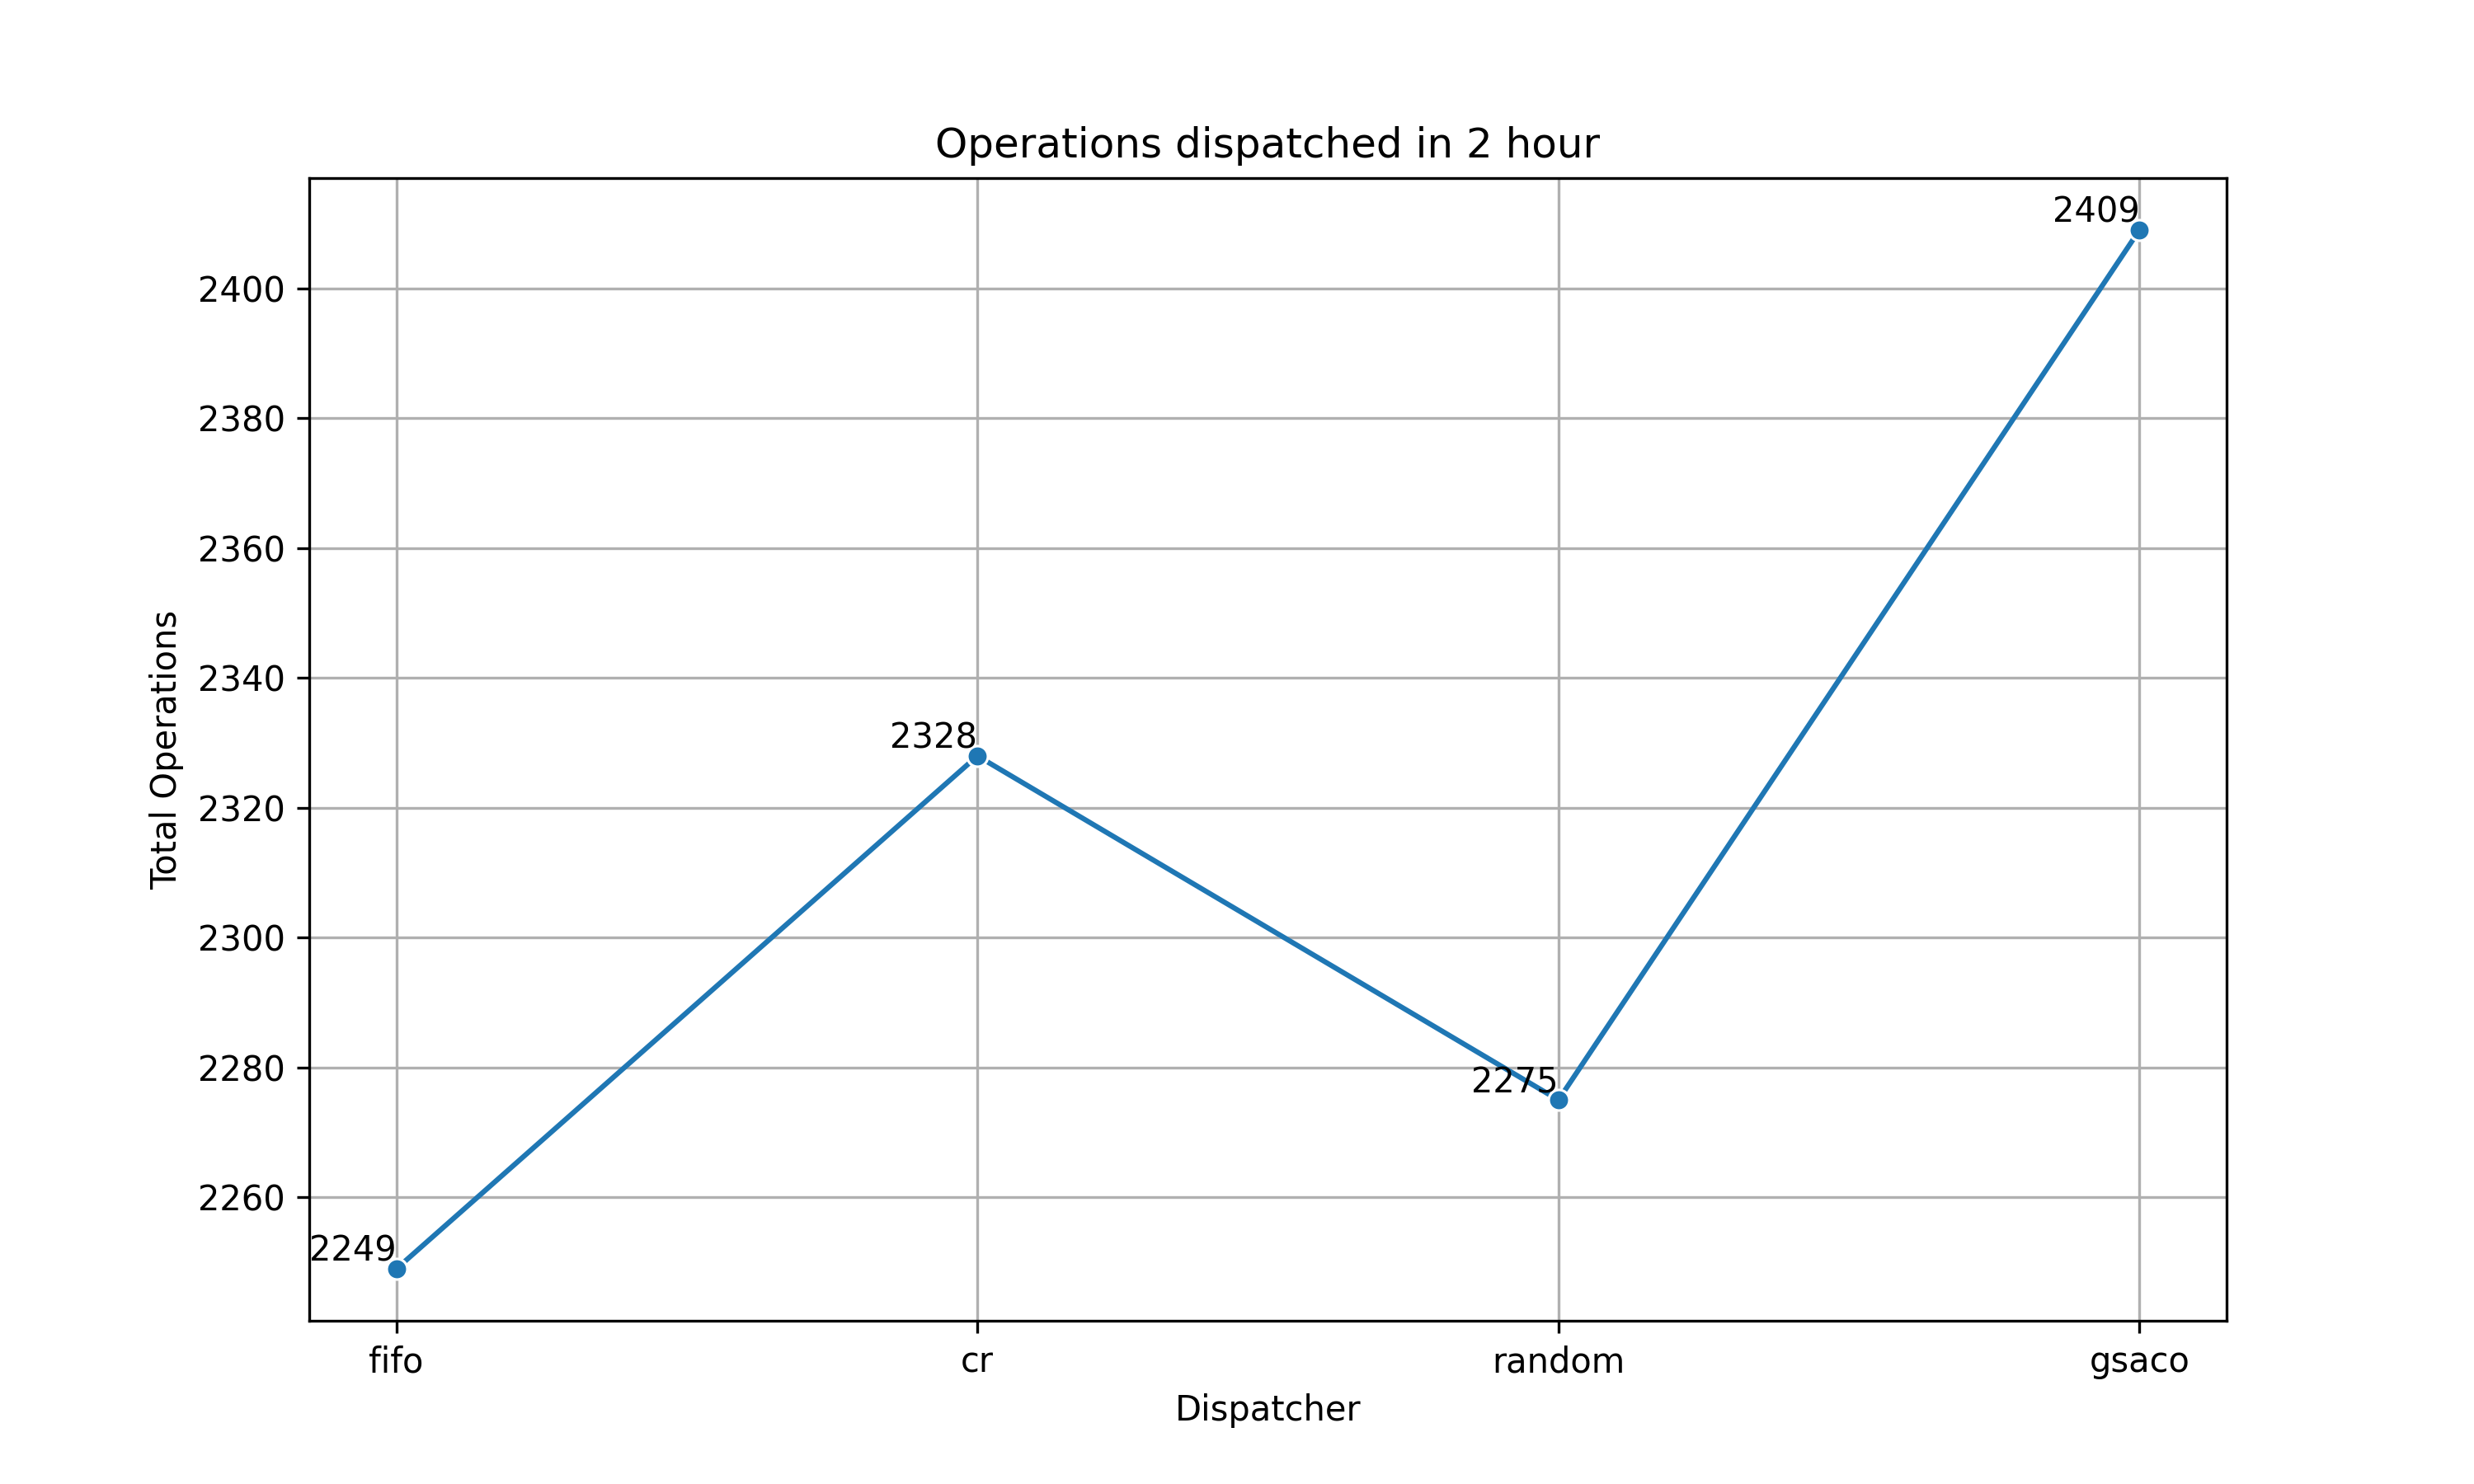
\includegraphics[width=\textwidth]{LVHM/total_operations_7200s.png}
		% \caption{}
		% \label{fig:oo2}
	\end{subfigure}\hfill
	\begin{subfigure}{0.32\textwidth}
		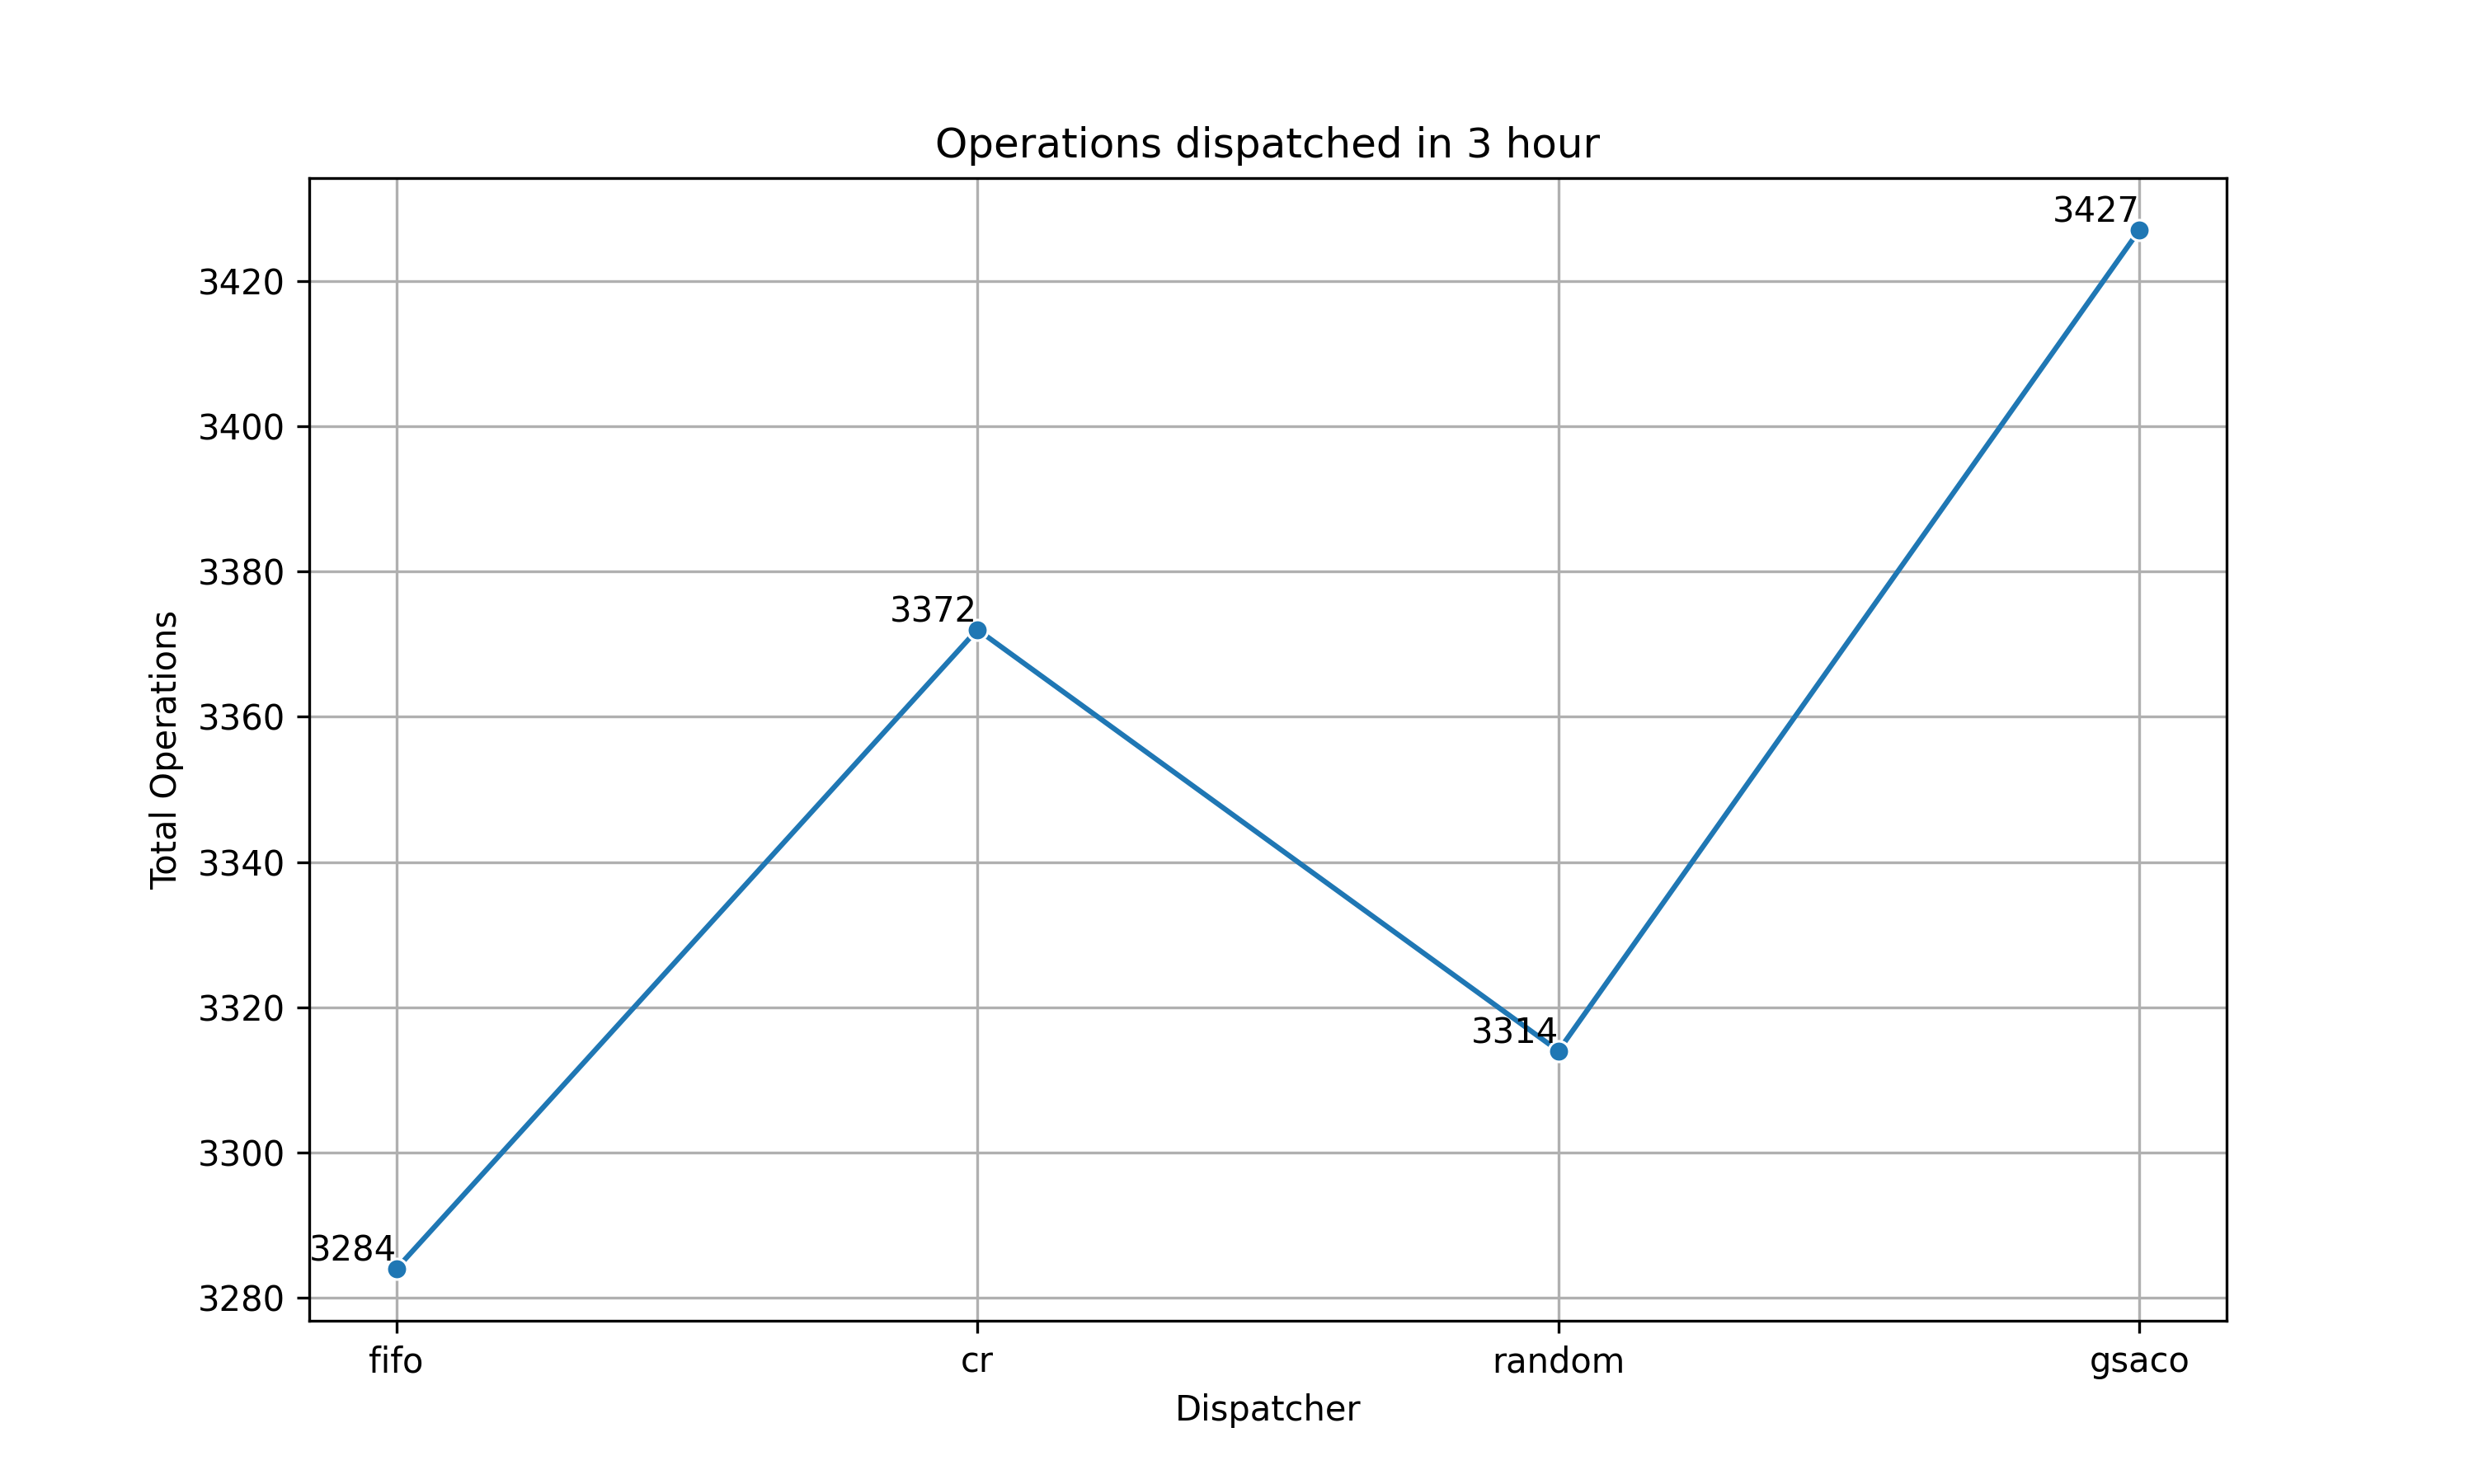
\includegraphics[width=\textwidth]{LVHM/total_operations_10800s.png}
		% \caption{}
		% \label{fig:oo3}
	\end{subfigure}
	\begin{subfigure}{0.32\textwidth}
		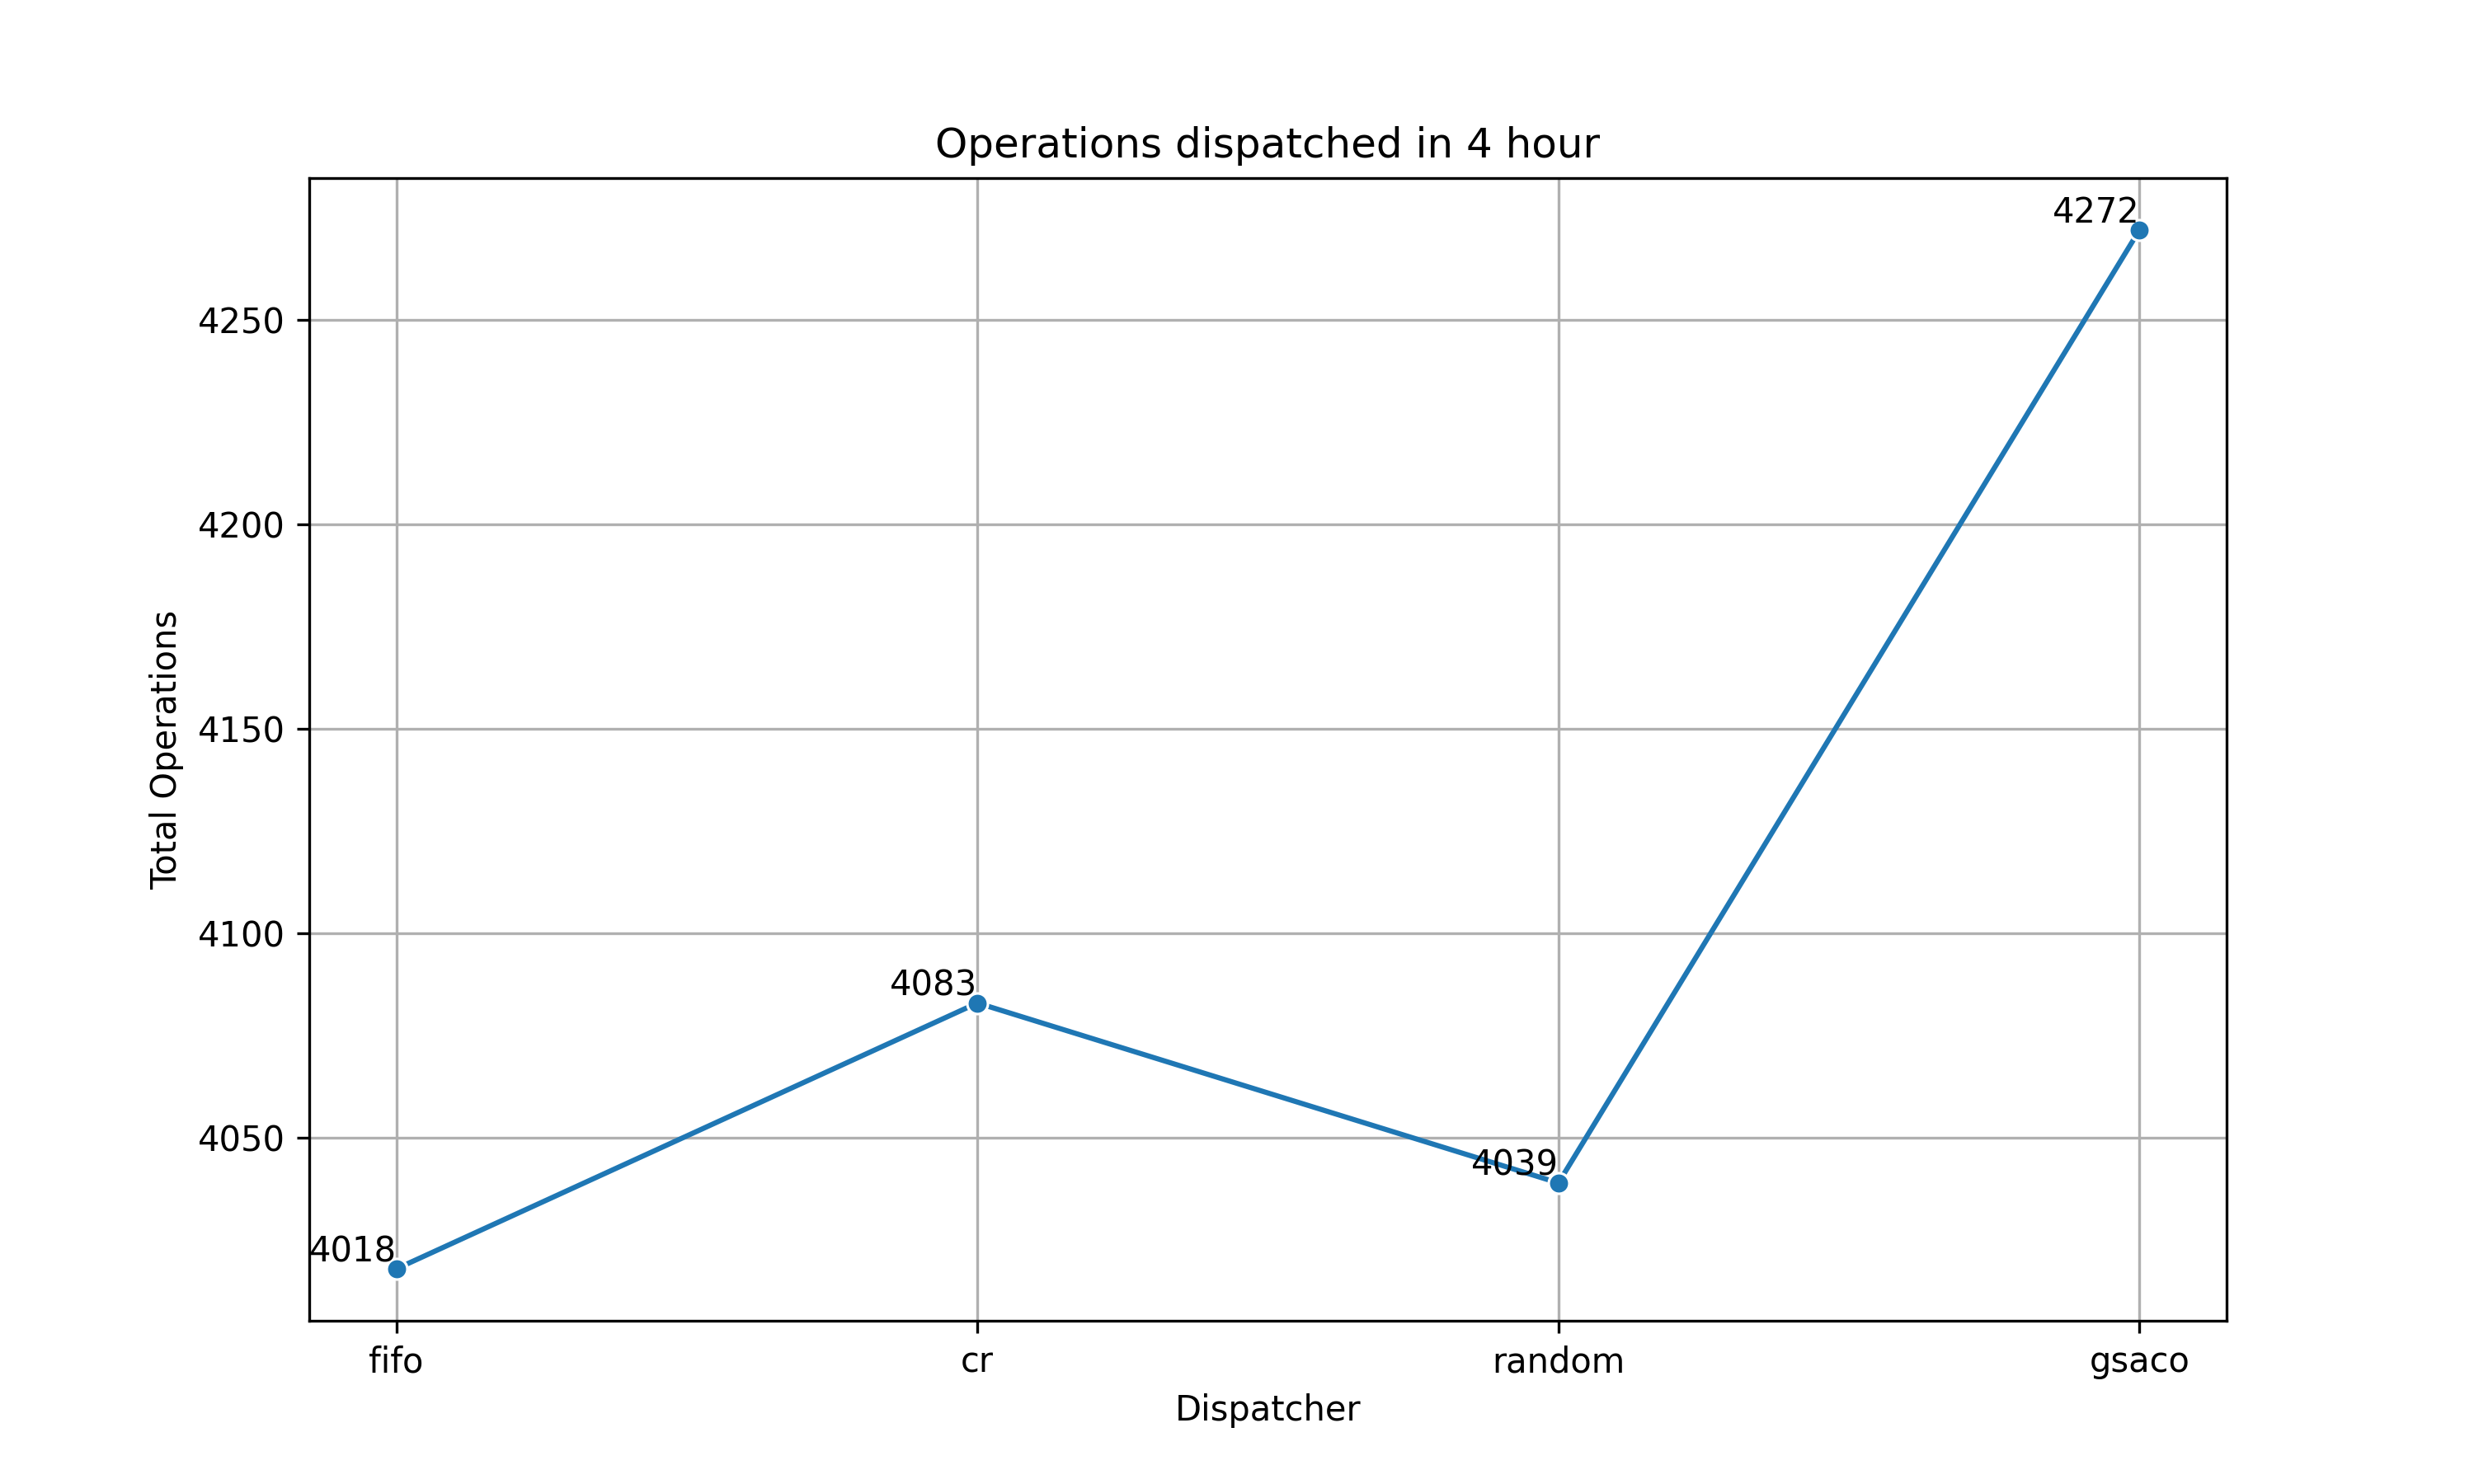
\includegraphics[width=\textwidth]{LVHM/total_operations_14400s.png}
		% \caption{}
		% \label{fig:oo4}
	\end{subfigure}\hfill
	\begin{subfigure}{0.32\textwidth}
		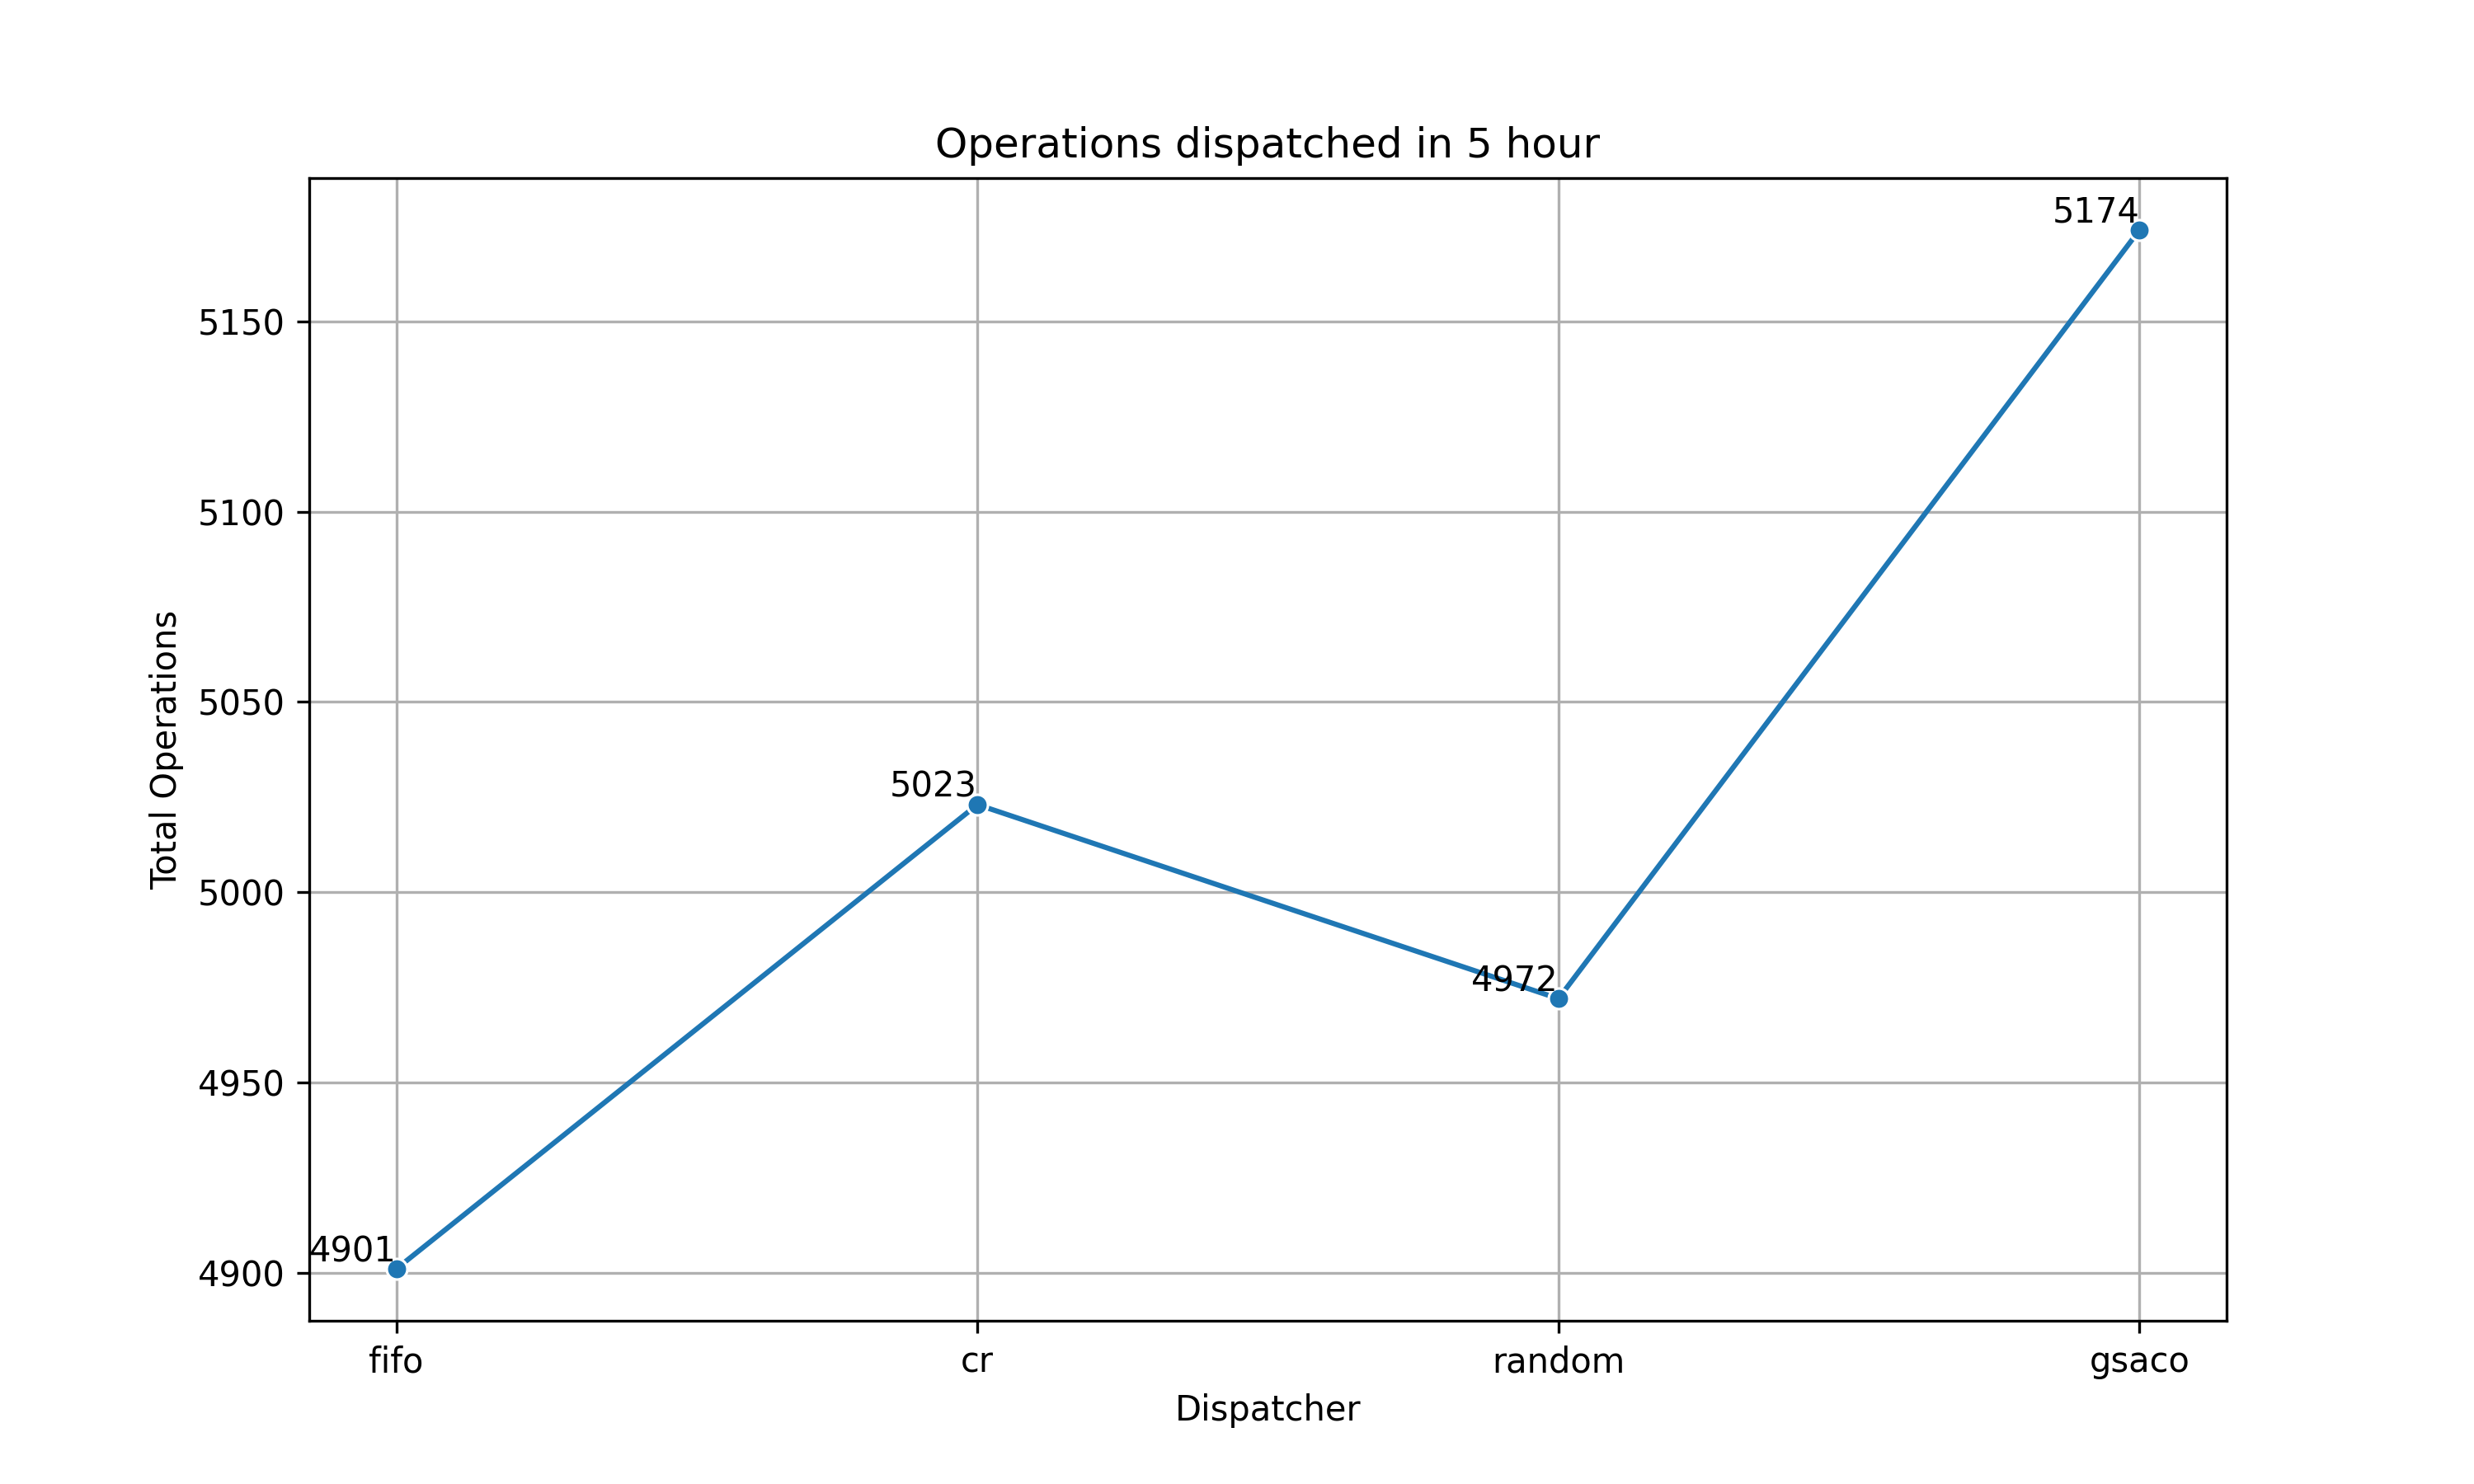
\includegraphics[width=\textwidth]{LVHM/total_operations_18000s.png}
		% \caption{}
		% \label{fig:oo5}
	\end{subfigure}\hfill
	\begin{subfigure}{0.32\textwidth}
		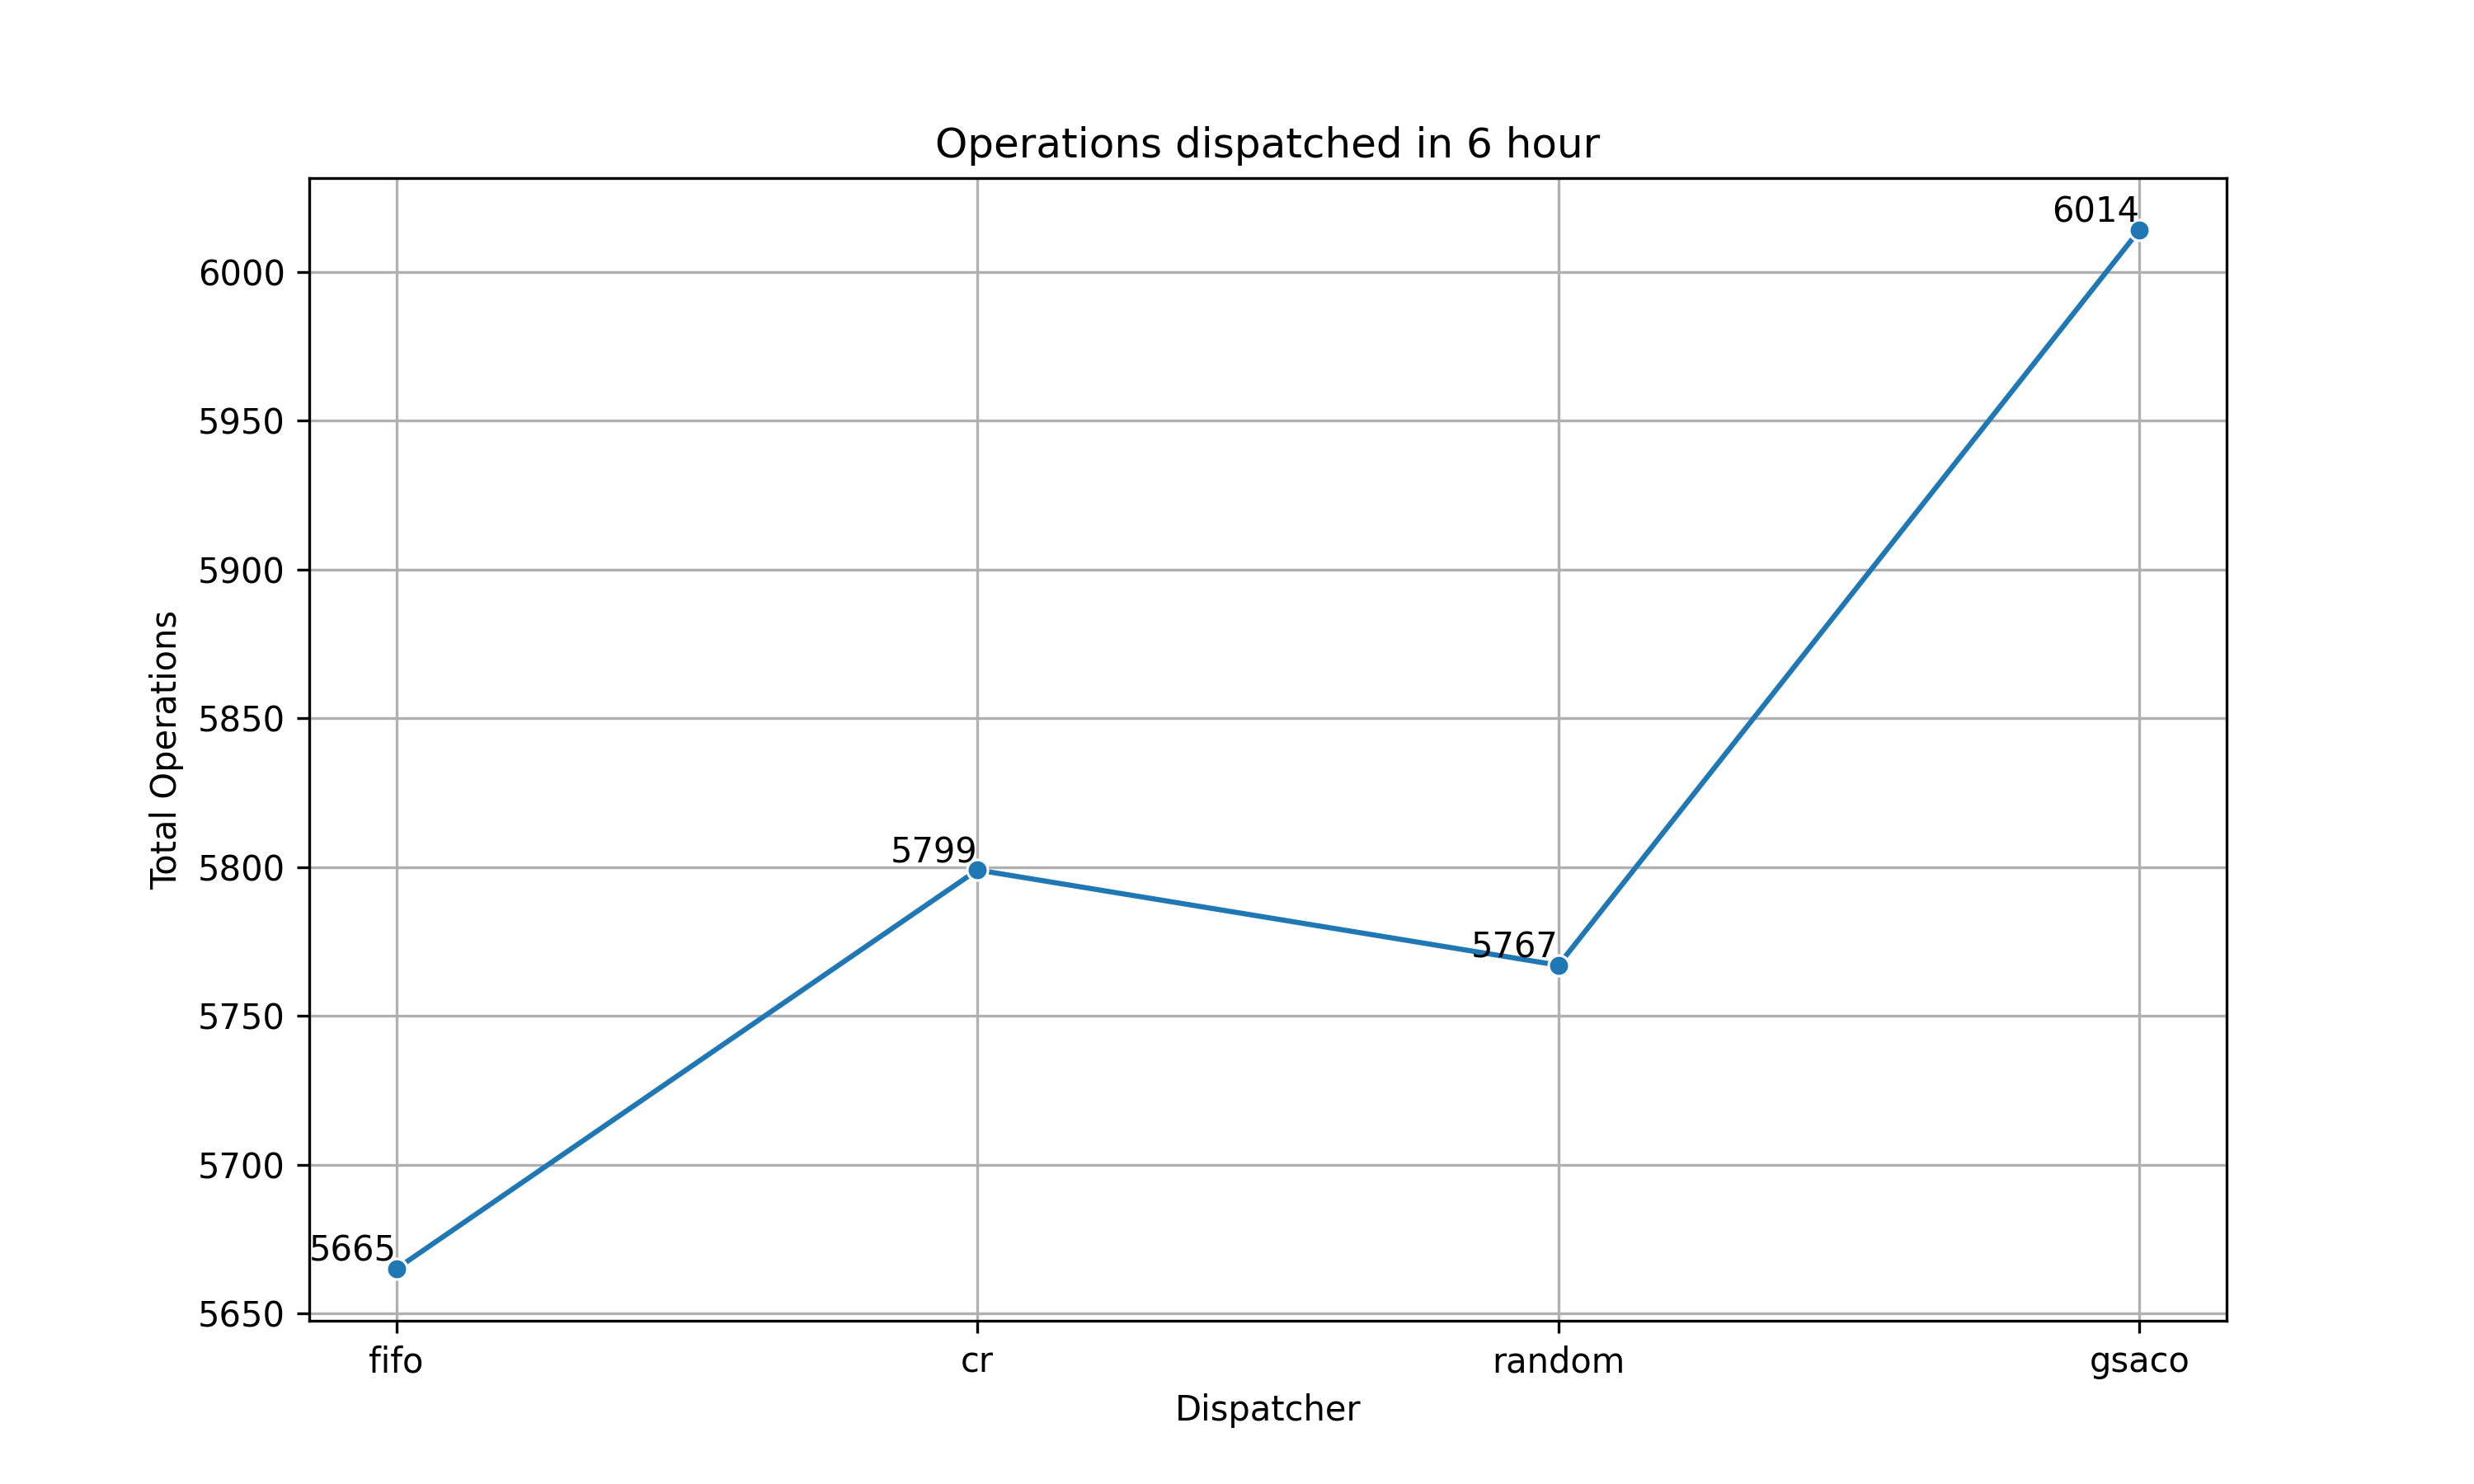
\includegraphics[width=\textwidth]{LVHM/total_operations_21600s.png}
		% \caption{}
		% \label{fig:oo6}
	\end{subfigure}
	\caption{Total operations completed LV/HM}
	\label{fig:totalopsLVHM}
\end{figure}

\begin{figure}[t]
	\centering
	\begin{subfigure}{0.32\textwidth}
		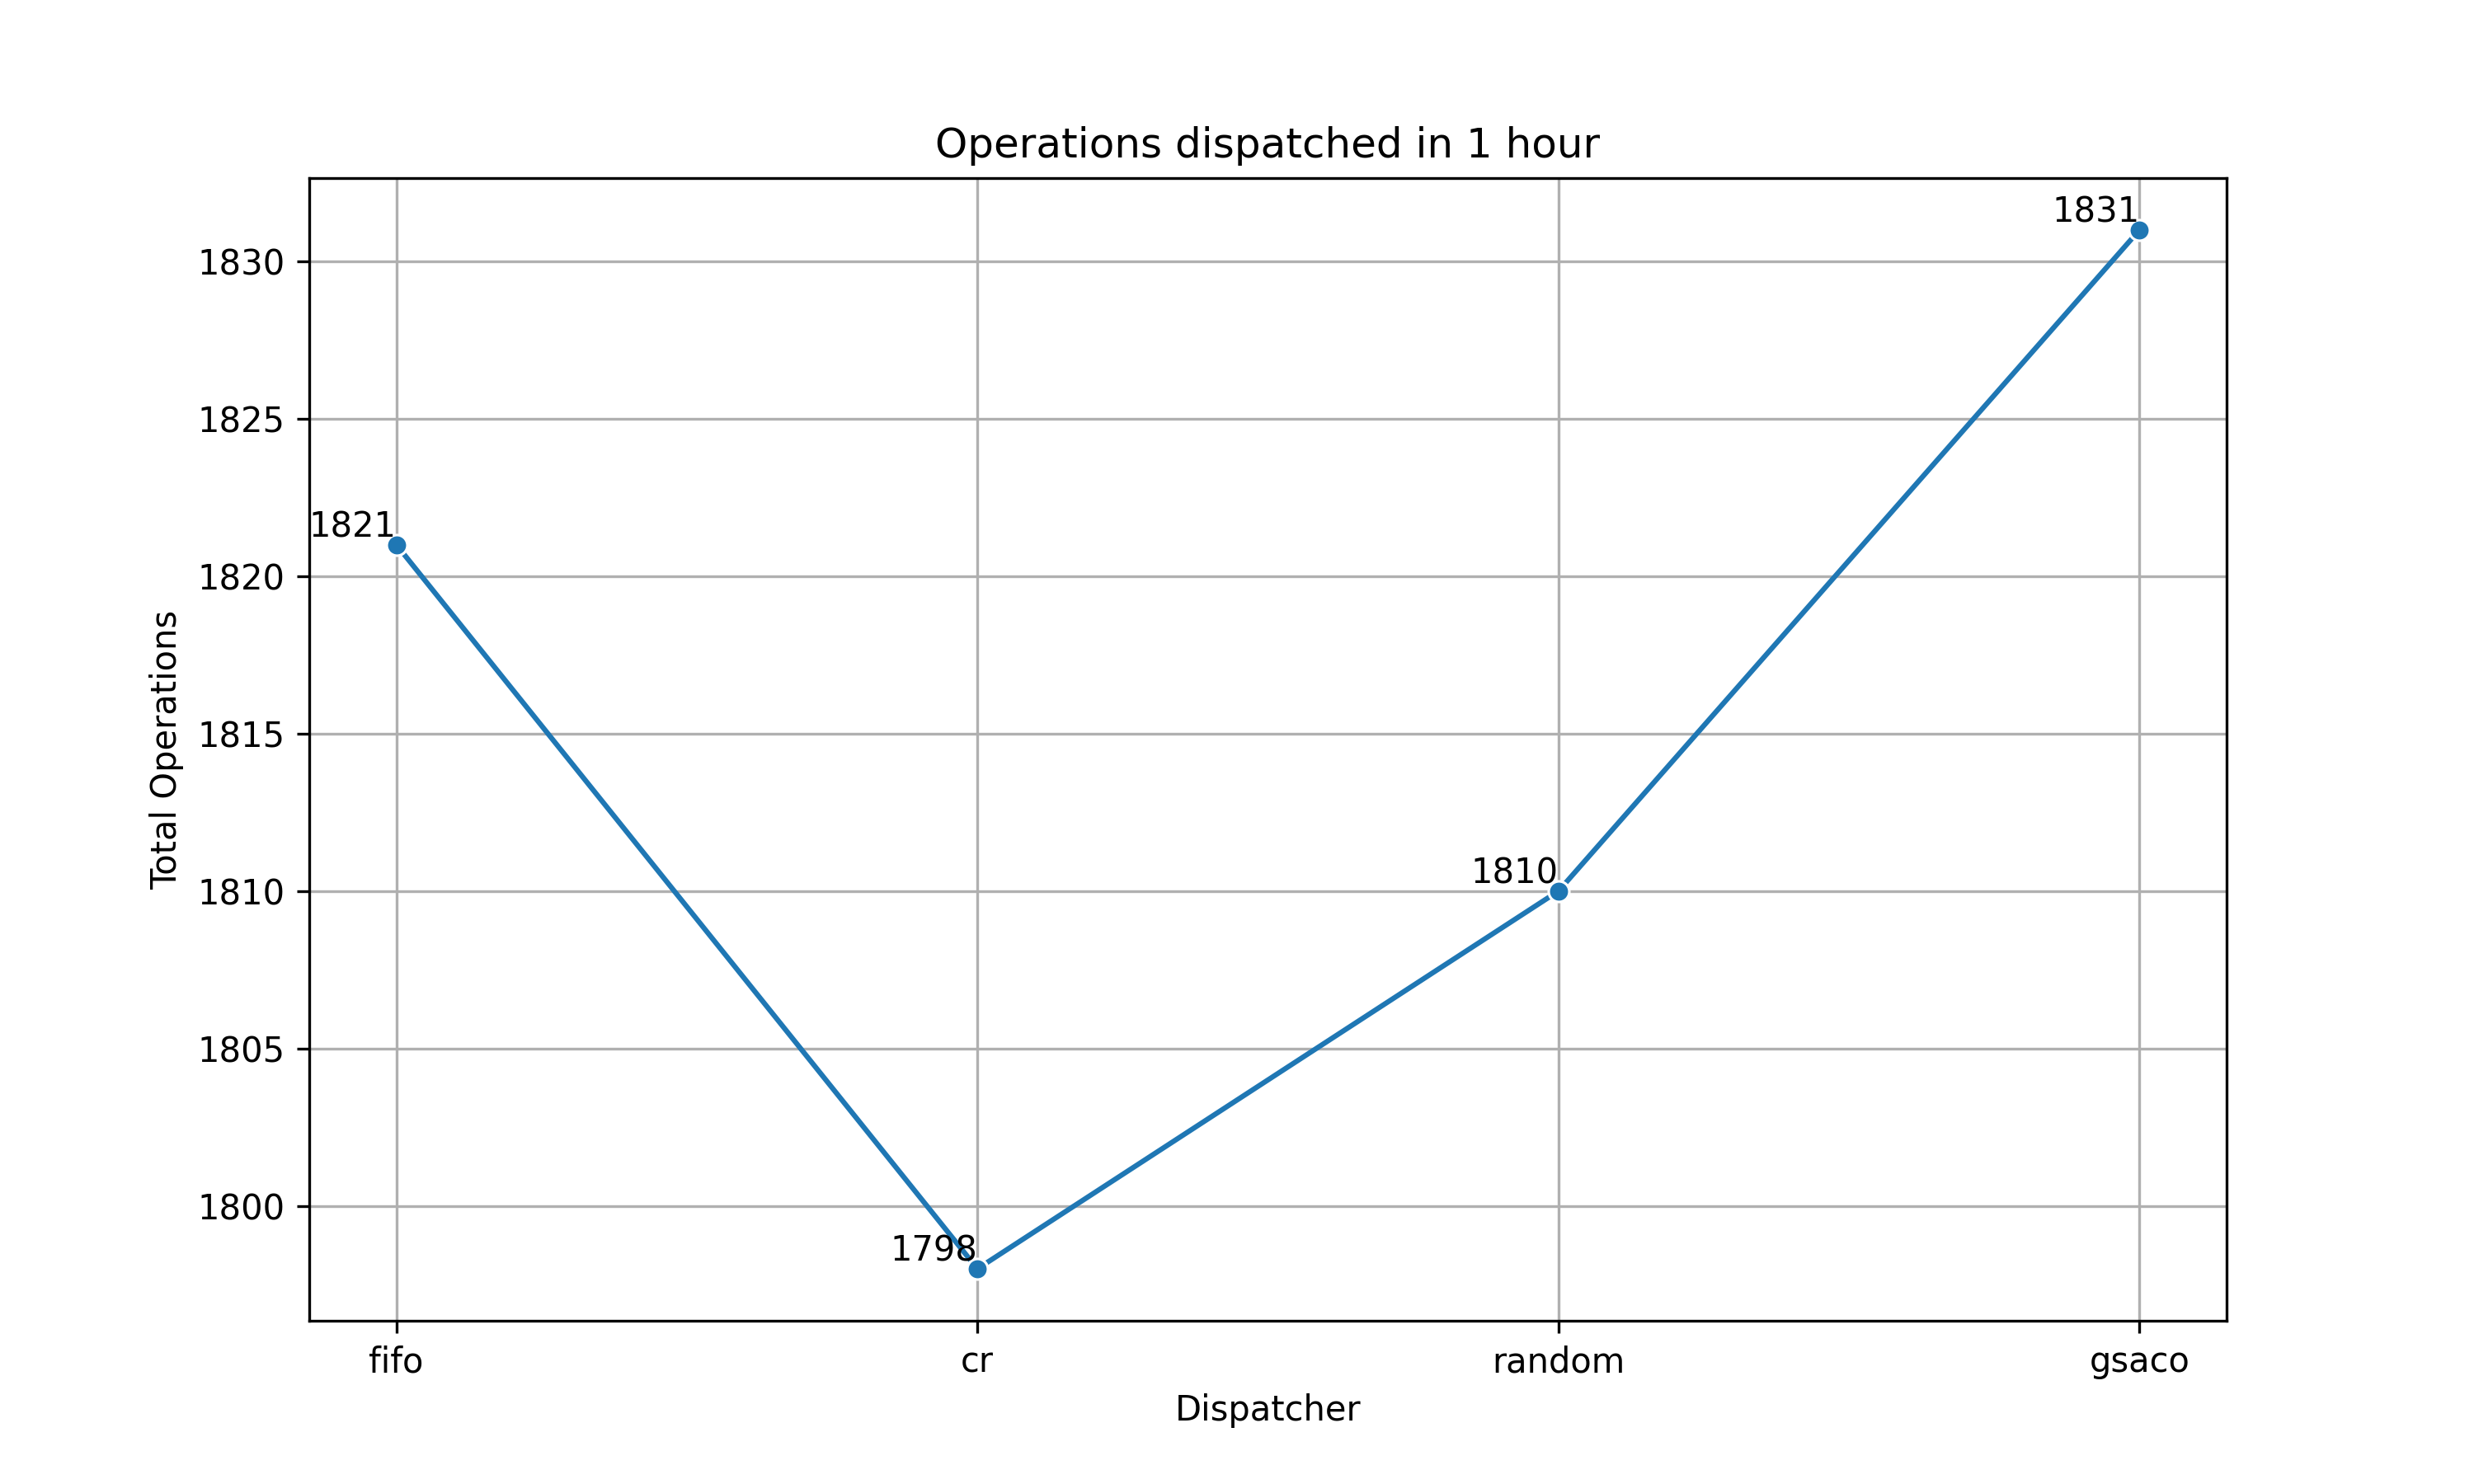
\includegraphics[width=\textwidth]{HVLM/total_operations_3600s.png}
		% \caption{}
		% \label{fig:o1}
	\end{subfigure}\hfill
	\begin{subfigure}{0.32\textwidth}
		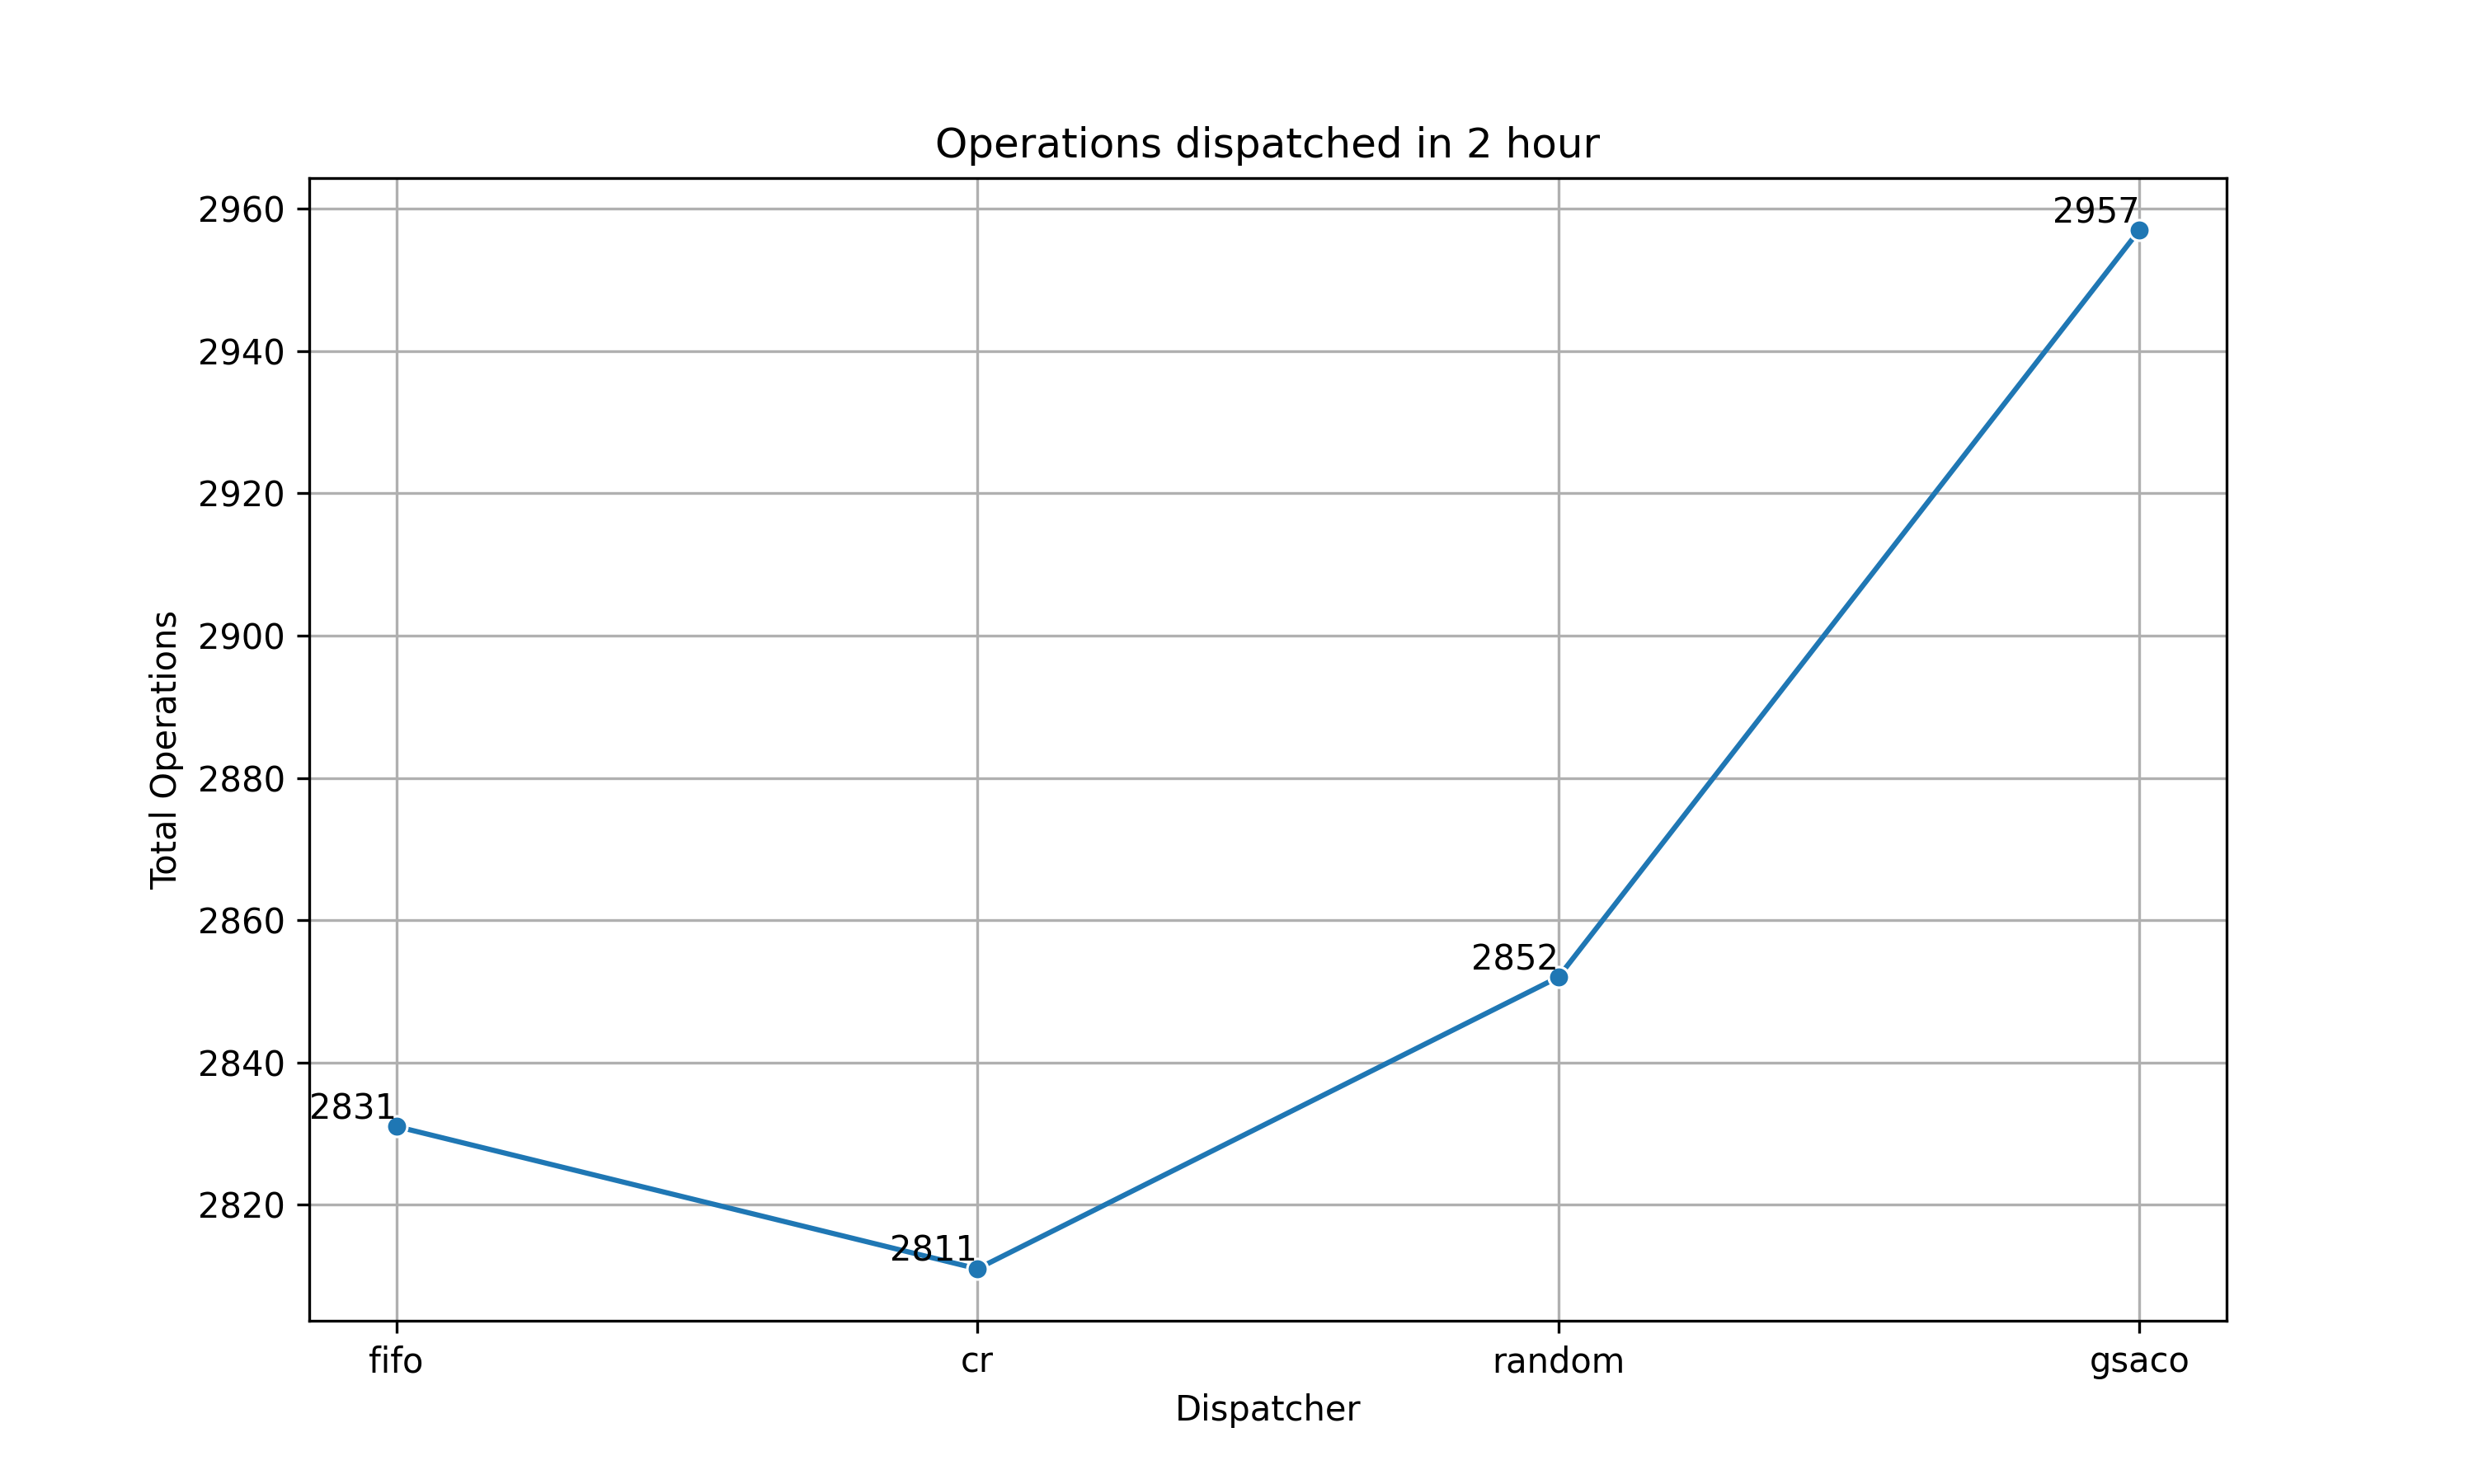
\includegraphics[width=\textwidth]{HVLM/total_operations_7200s.png}
		% \caption{}
		% \label{fig:o2}
	\end{subfigure}\hfill
	\begin{subfigure}{0.32\textwidth}
		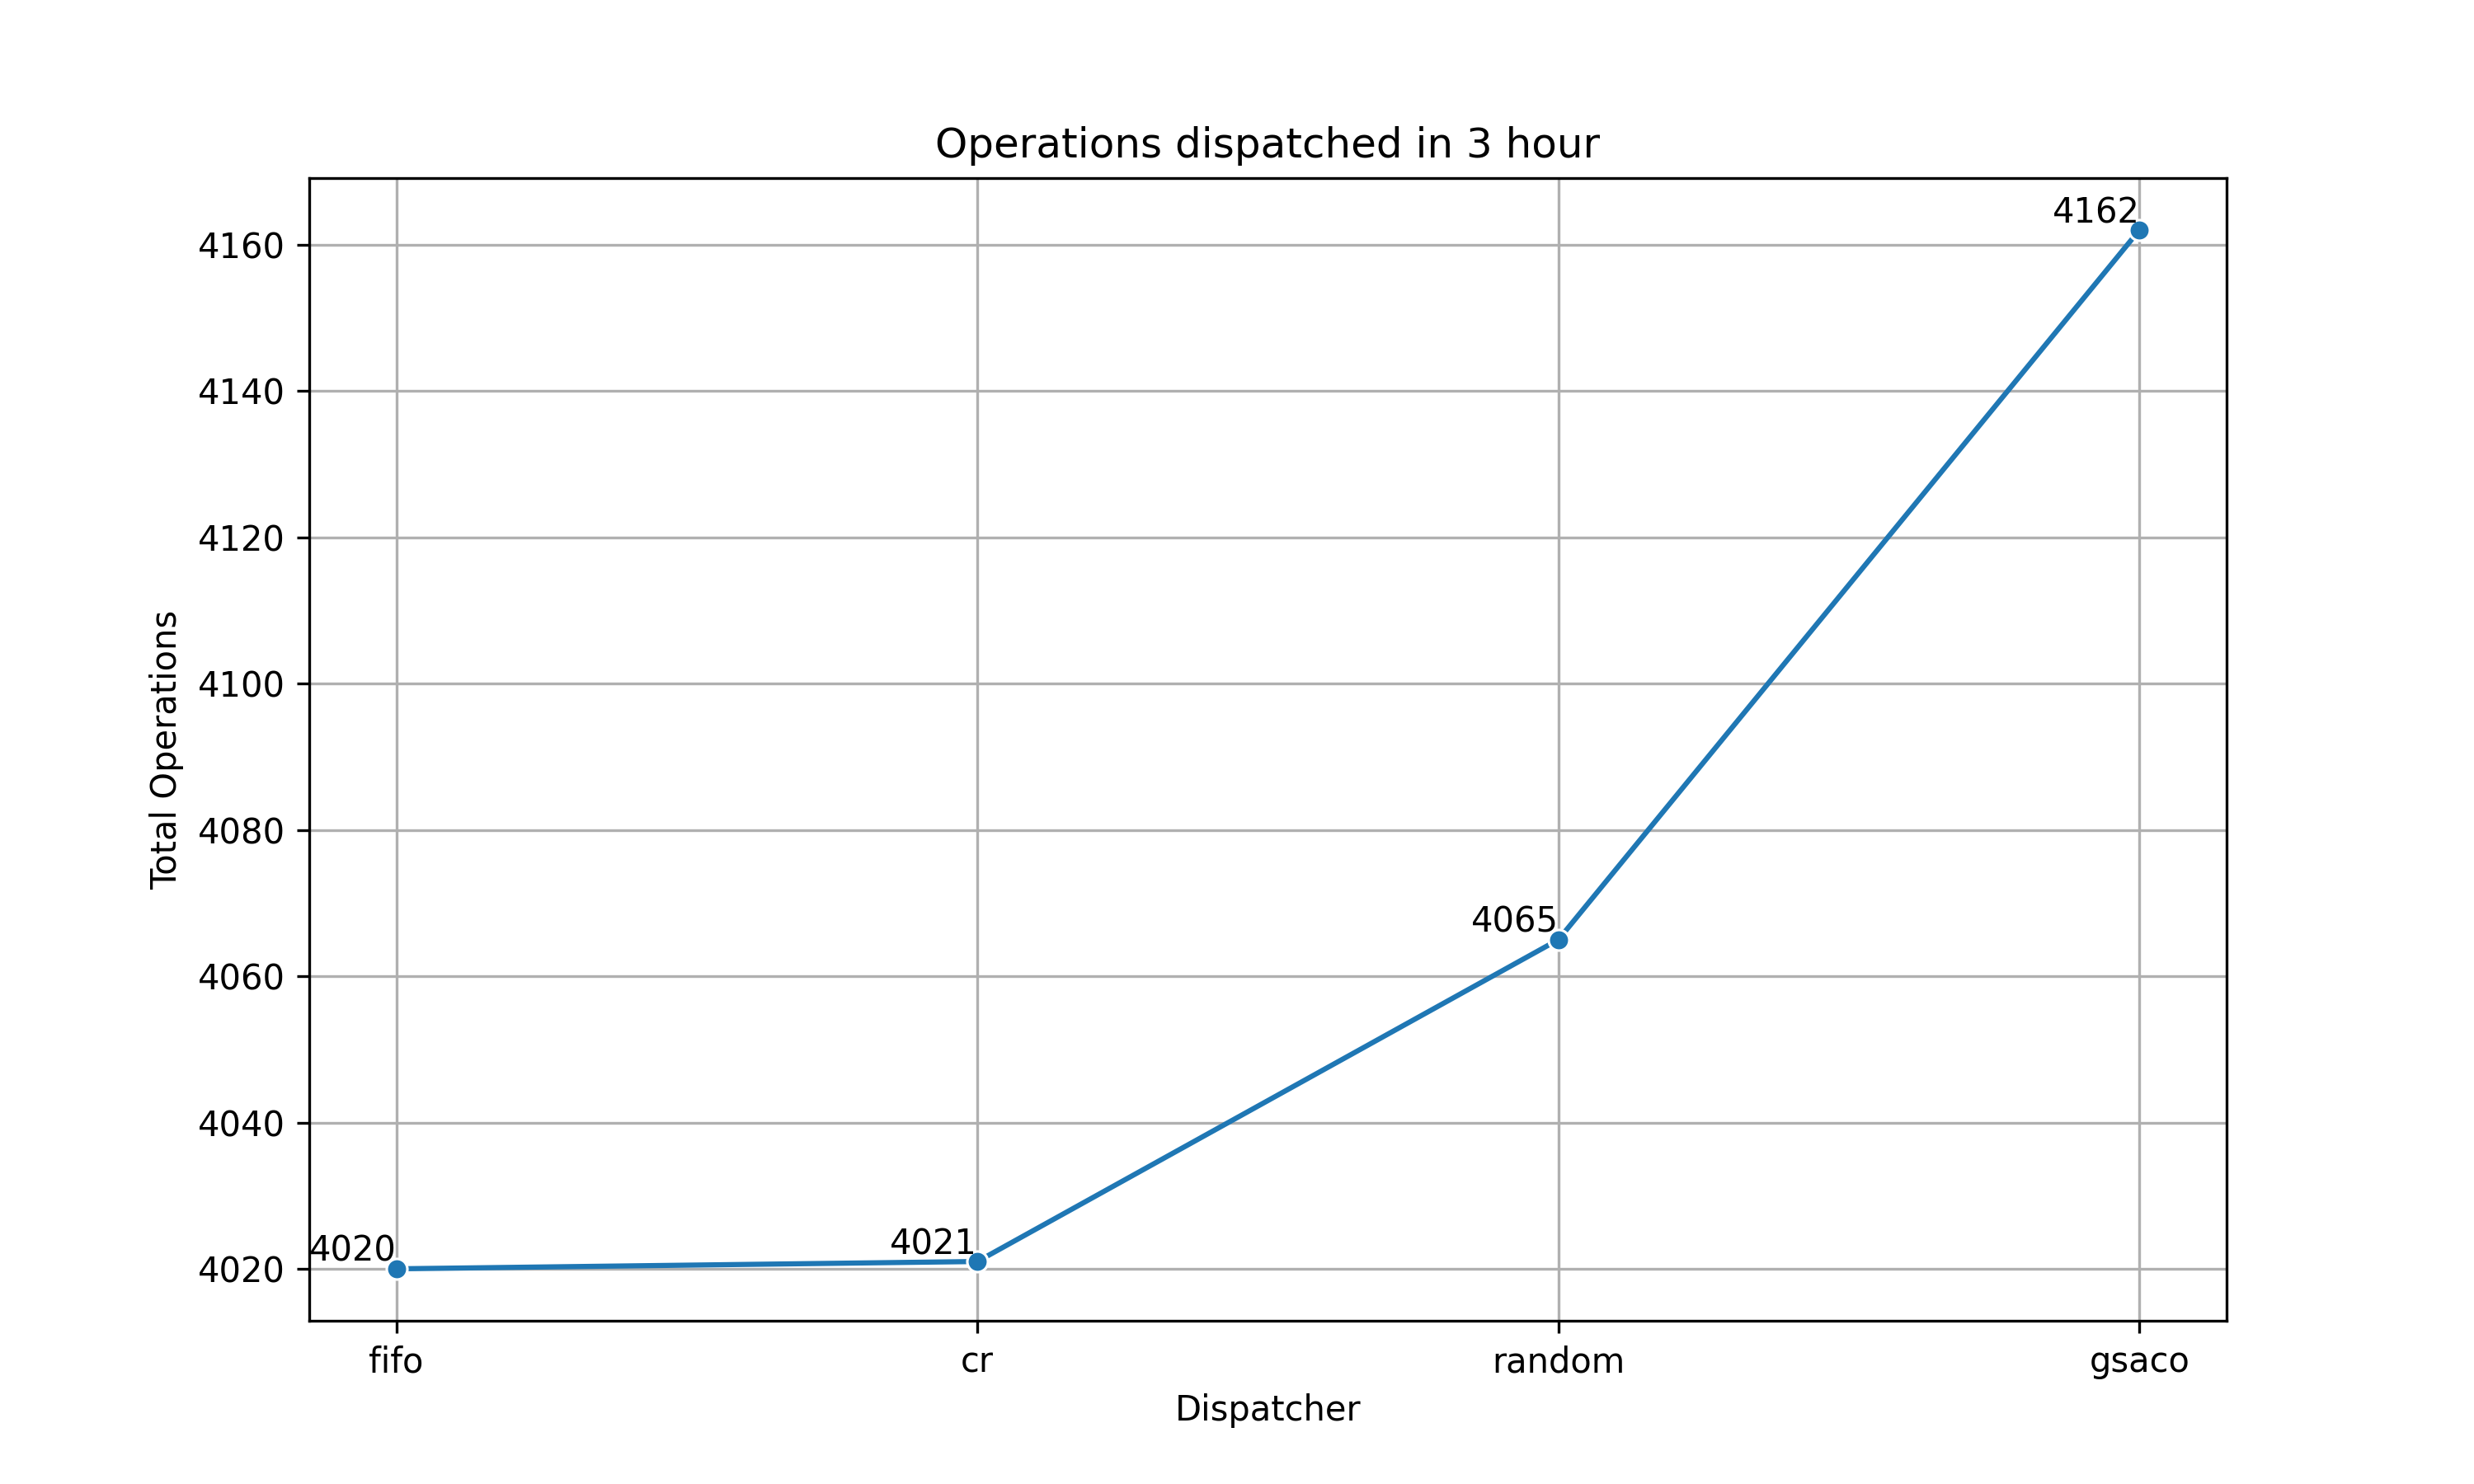
\includegraphics[width=\textwidth]{HVLM/total_operations_10800s.png}
		% \caption{}
		% \label{fig:o3}
	\end{subfigure}
	\begin{subfigure}{0.32\textwidth}
		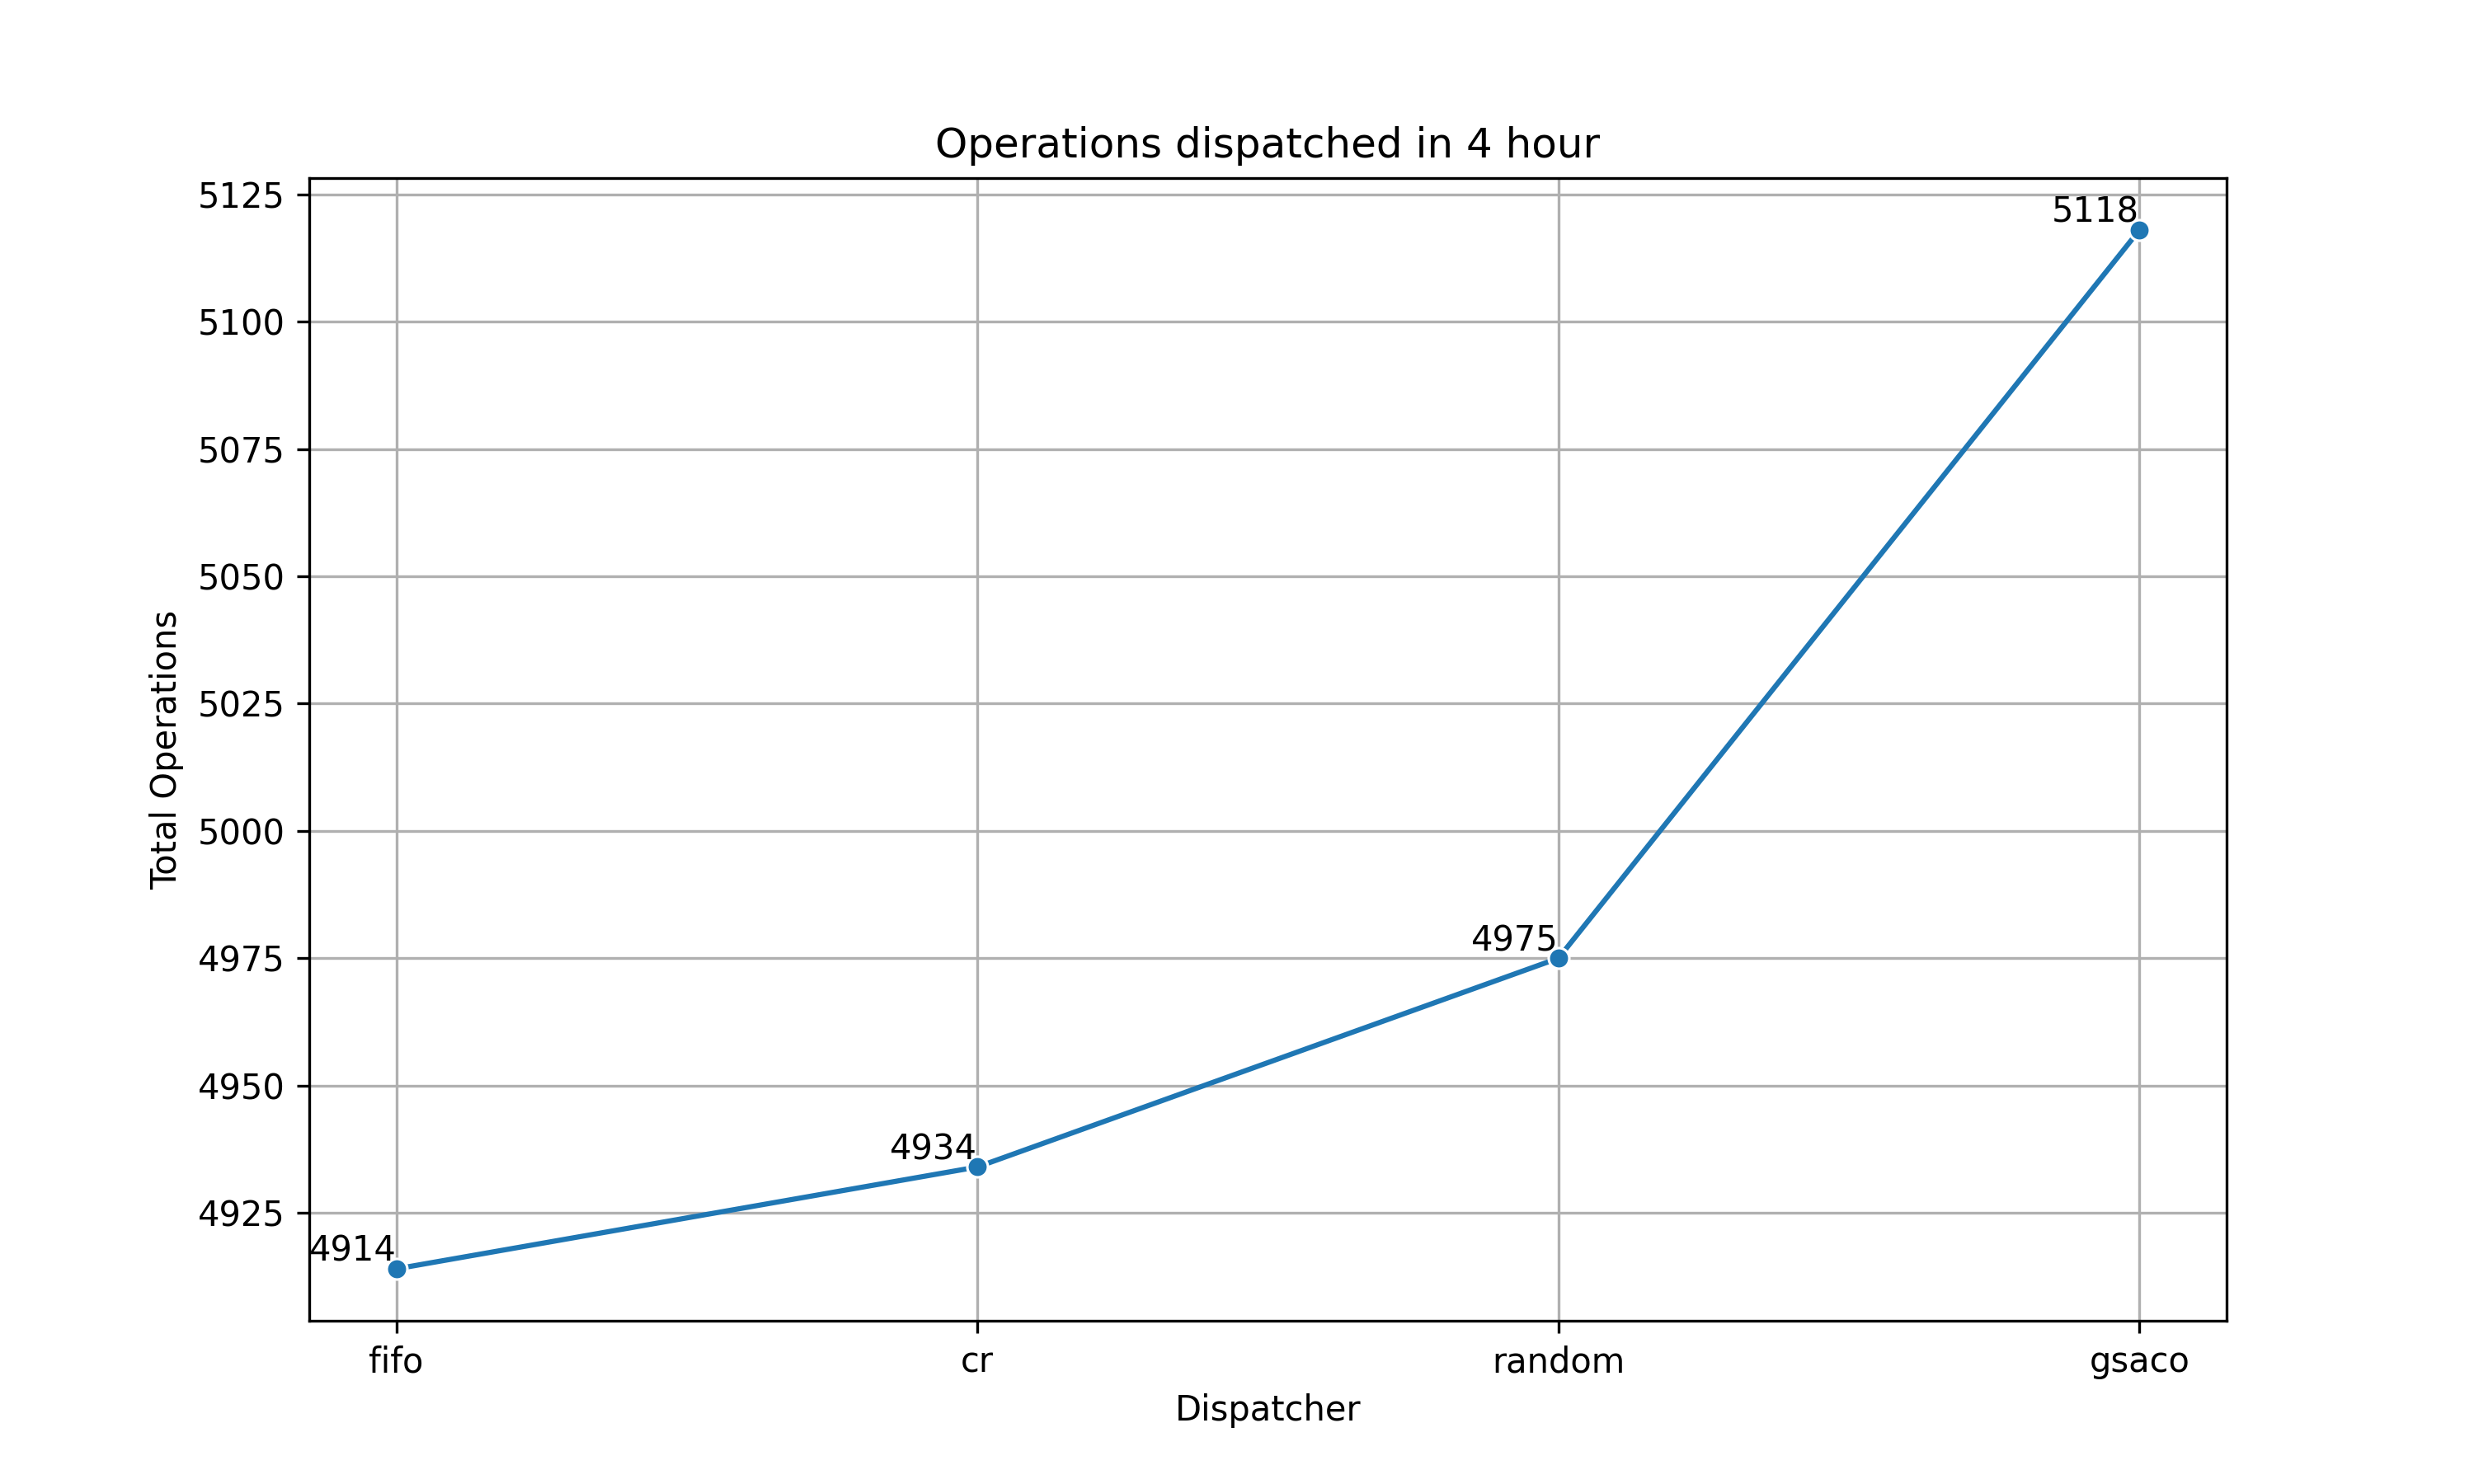
\includegraphics[width=\textwidth]{HVLM/total_operations_14400s.png}
		% \caption{}
		% \label{fig:o4}
	\end{subfigure}\hfill
	\begin{subfigure}{0.32\textwidth}
		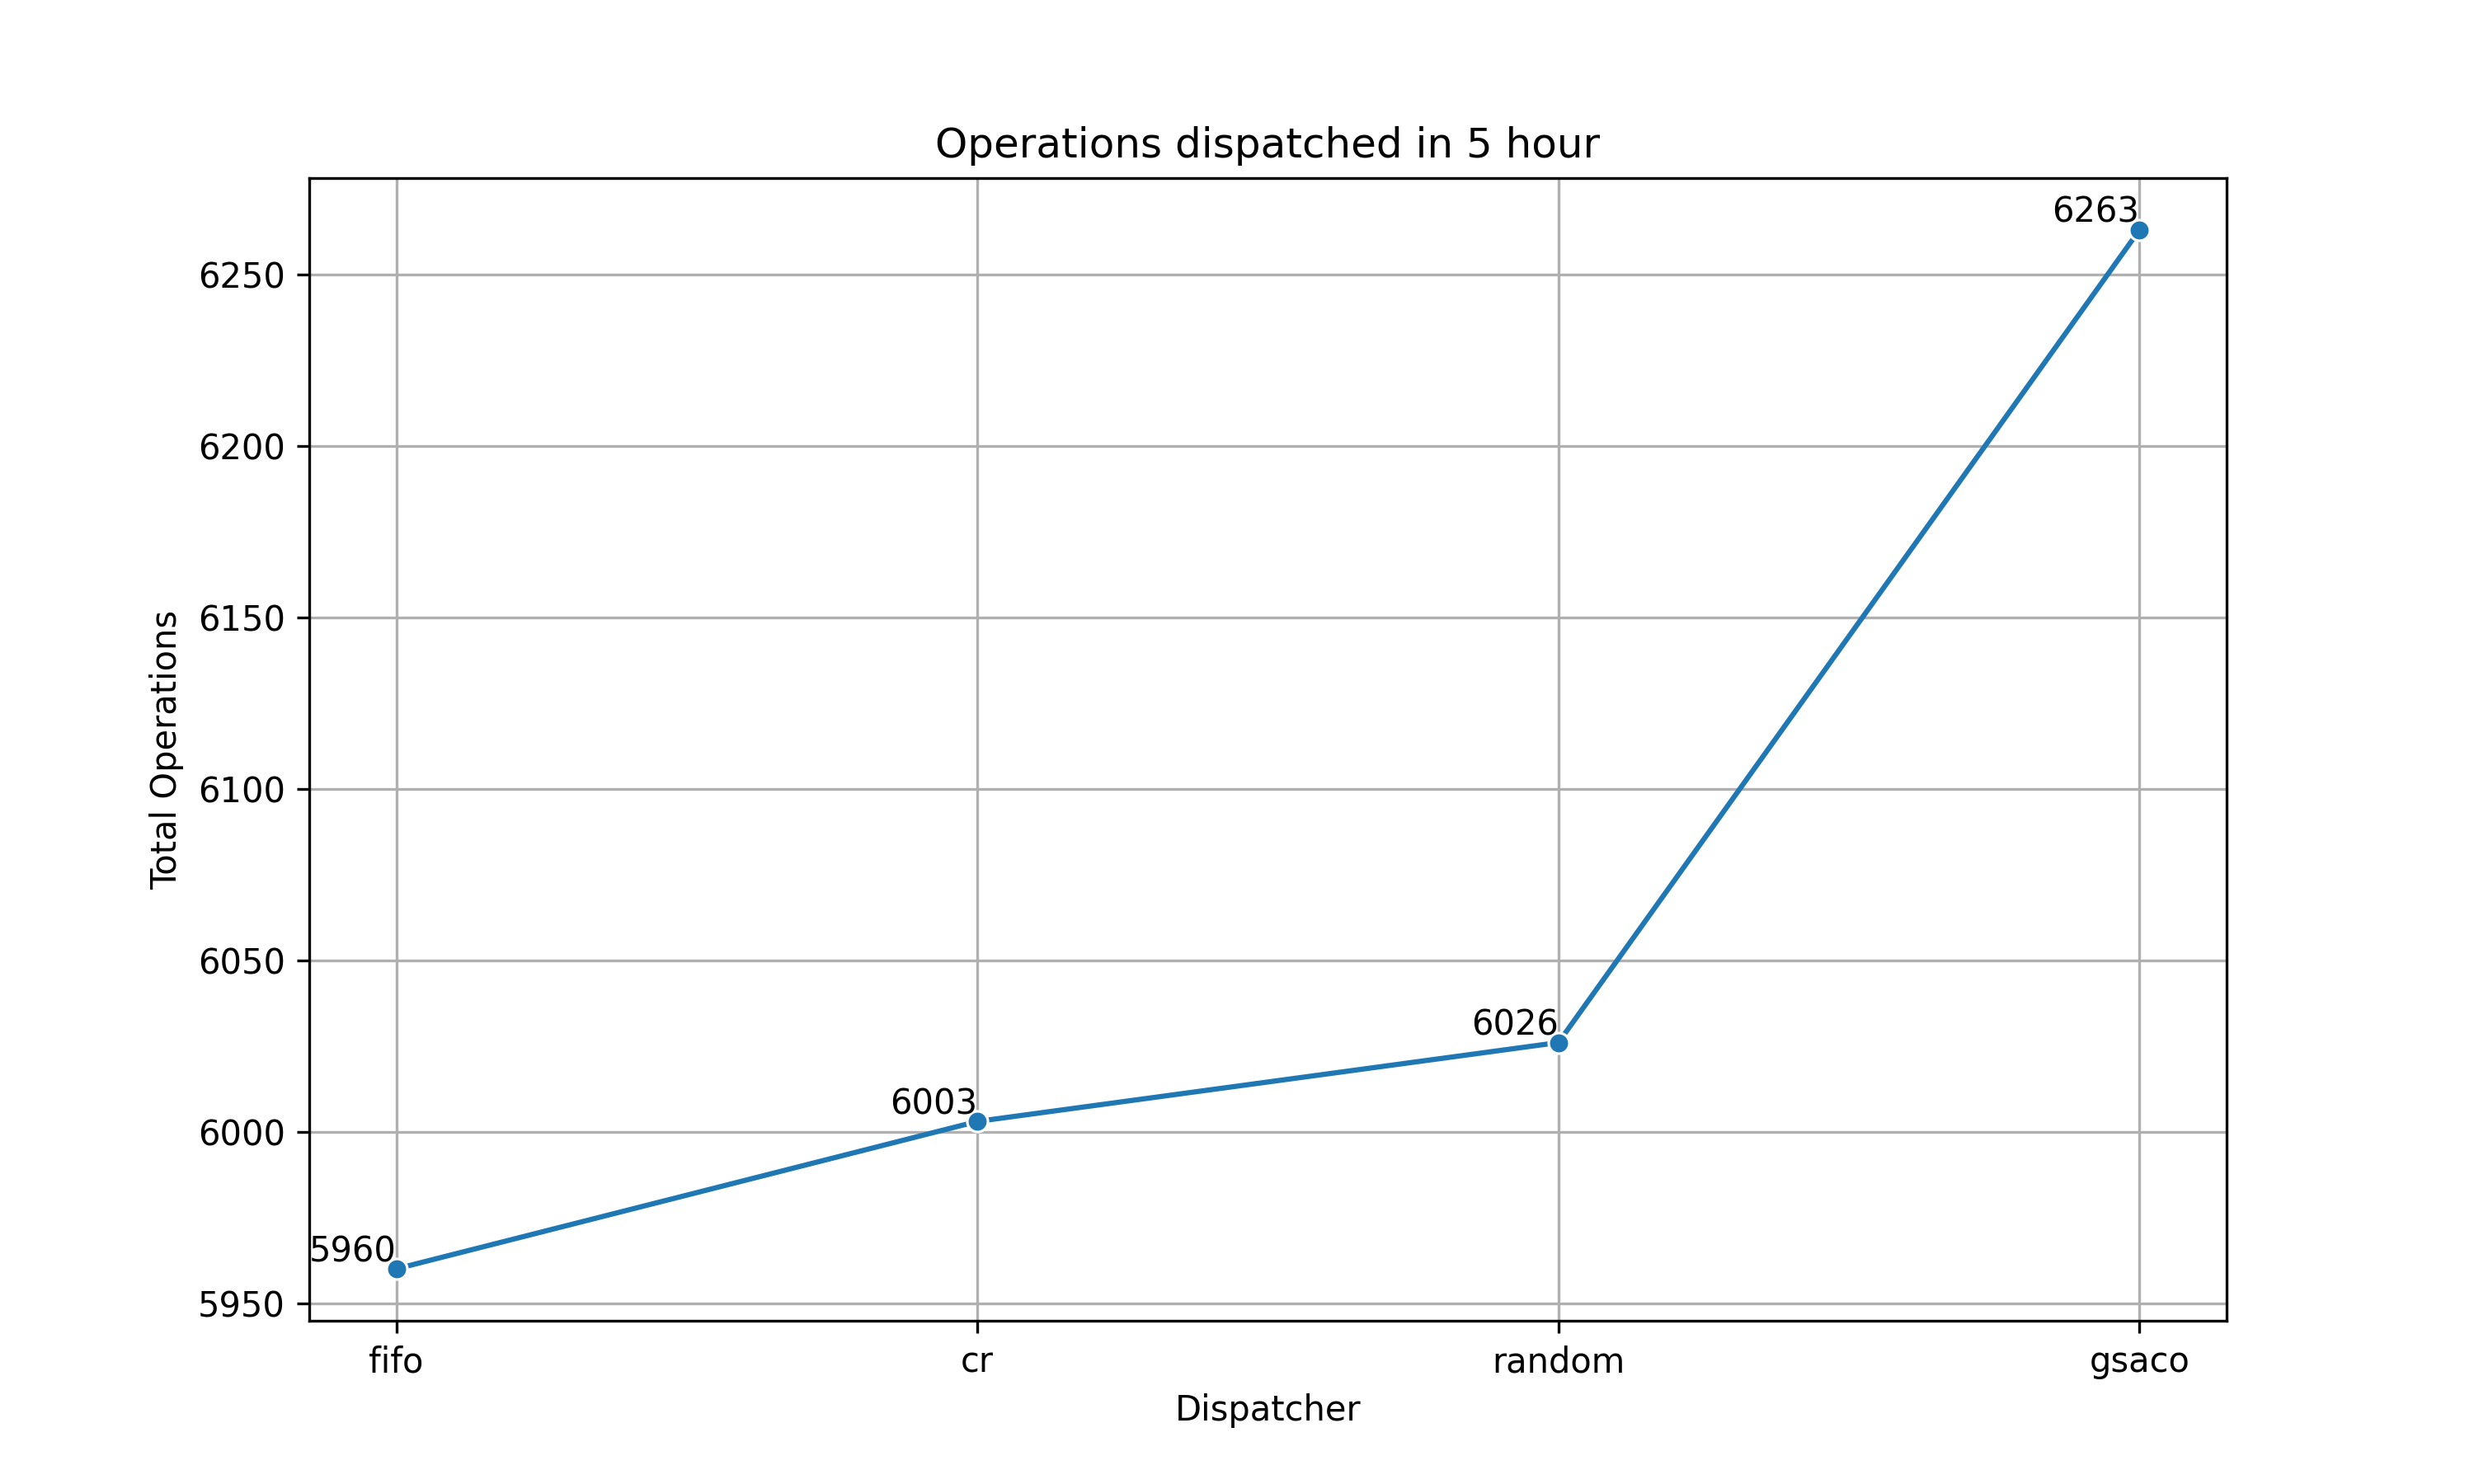
\includegraphics[width=\textwidth]{HVLM/total_operations_18000s.png}
		% \caption{}
		% \label{fig:o5}
	\end{subfigure}\hfill
	\begin{subfigure}{0.32\textwidth}
		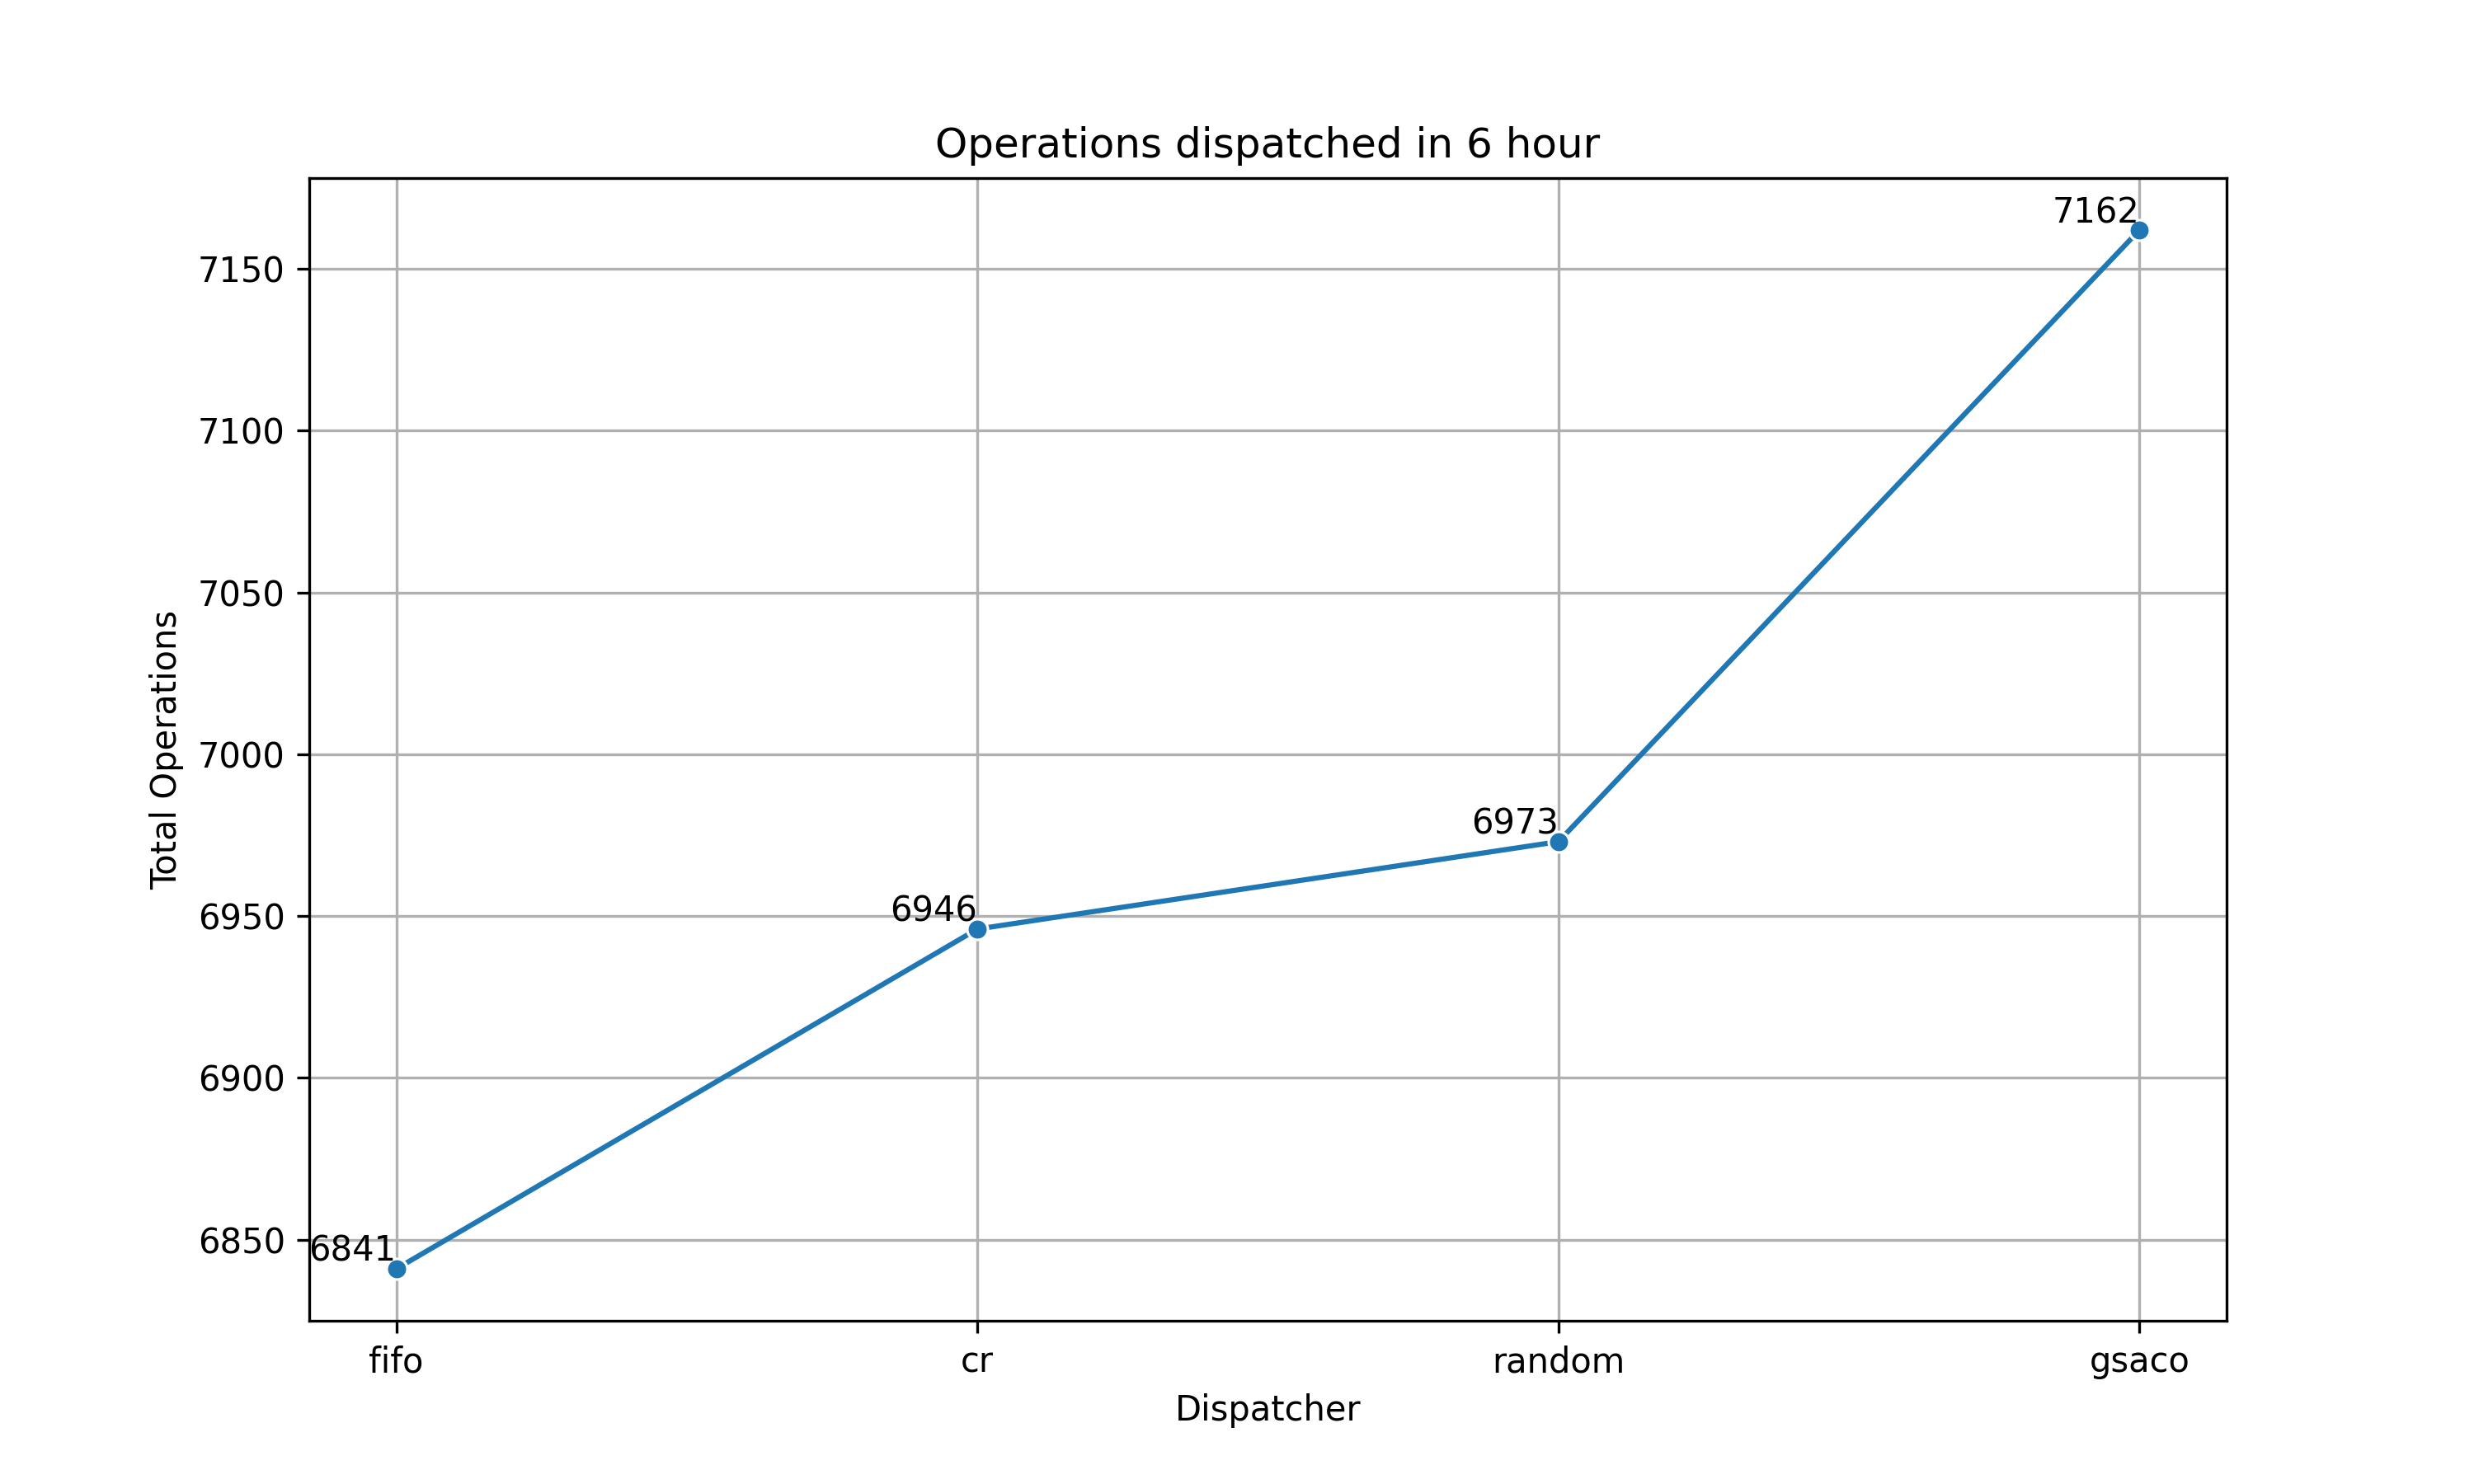
\includegraphics[width=\textwidth]{HVLM/total_operations_21600s.png}
		% \caption{}
		% \label{fig:o6}
	\end{subfigure}
	\caption{Completed operations for HV/LM}
	\label{fig:totalopsHVLM}
\end{figure}